% ============================================================
%  Documentación Proyecto Final — Aplicación Web de Cuestionarios
%  Compilar en Overleaf (pdflatex)
% ============================================================
\documentclass[12pt,a4paper]{article}

\usepackage[utf8]{inputenc}
\usepackage[spanish]{babel}
\usepackage[T1]{fontenc}
\usepackage{lmodern}
\usepackage{graphicx}
\usepackage[margin=2.5cm]{geometry}
\usepackage{hyperref}
\usepackage{booktabs}
\usepackage{longtable}
\usepackage{array}
\usepackage{xcolor}
\usepackage{listings}
\usepackage{tikz}
\usepackage{float}
\usepackage{enumitem}
\usepackage{fancyhdr}
\usepackage{parskip}
\usepackage{multirow}
\usepackage{tabularx}
\usepackage{mdframed}

\usetikzlibrary{shapes.geometric, arrows.meta, positioning, calc, fit, backgrounds}

% ── Colores ──────────────────────────────────────────────────
\definecolor{primary}{RGB}{79,70,229}
\definecolor{codebg}{RGB}{248,248,248}
\definecolor{codeframe}{RGB}{200,200,200}
\definecolor{httpget}{RGB}{34,197,94}
\definecolor{httppost}{RGB}{59,130,246}
\definecolor{httppatch}{RGB}{234,179,8}
\definecolor{httpput}{RGB}{249,115,22}
\definecolor{rowgray}{RGB}{245,245,250}

% ── Listings ─────────────────────────────────────────────────
\lstset{
  backgroundcolor=\color{codebg},
  basicstyle=\ttfamily\small,
  breaklines=true,
  frame=single,
  rulecolor=\color{codeframe},
  keywordstyle=\color{primary}\bfseries,
  stringstyle=\color{teal},
  commentstyle=\color{gray}\itshape,
  showstringspaces=false,
  xleftmargin=8pt,
  xrightmargin=8pt,
  aboveskip=8pt,
  belowskip=8pt,
}

% ── Hyperref ─────────────────────────────────────────────────
\hypersetup{
  colorlinks=true,
  linkcolor=primary,
  urlcolor=primary,
  citecolor=primary,
  pdftitle={Documentación Proyecto Final — Aplicación Web de Cuestionarios},
}

% ── Cabecera / pie ───────────────────────────────────────────
\pagestyle{fancy}
\fancyhf{}
\rhead{\small Aplicación Web de Cuestionarios — Proyecto Final}
\lhead{\small IIMAS -- UNAM}
\cfoot{\thepage}
\renewcommand{\headrulewidth}{0.4pt}

% ── Comandos auxiliares ───────────────────────────────────────
\newcommand{\httpget}[1]{\colorbox{httpget!20}{\texttt{\textcolor{httpget!70!black}{GET}}} \texttt{#1}}
\newcommand{\httppost}[1]{\colorbox{httppost!20}{\texttt{\textcolor{httppost!70!black}{POST}}} \texttt{#1}}
\newcommand{\httpput}[1]{\colorbox{httpput!20}{\texttt{\textcolor{httpput!70!black}{PUT}}} \texttt{#1}}
\newcommand{\httppatch}[1]{\colorbox{httppatch!20}{\texttt{\textcolor{httppatch!70!black}{PATCH}}} \texttt{#1}}

% ── Entorno para notas ────────────────────────────────────────
\newmdenv[
  backgroundcolor=primary!6,
  linecolor=primary,
  linewidth=1.5pt,
  leftline=true, rightline=false, topline=false, bottomline=false,
  innerleftmargin=10pt, innerrightmargin=6pt,
  skipabove=6pt, skipbelow=6pt,
]{nota}

% =============================================================
\begin{document}

% ==================== PORTADA ================================
\begin{titlepage}
  \centering

  % Logos
  \begin{minipage}[c]{0.28\textwidth}
    \centering
    
\includegraphics[width=0.85\textwidth]{logo_iimas.png}
  \end{minipage}
  \hfill
  \begin{minipage}[c]{0.28\textwidth}
    \centering
    
\includegraphics[width=0.85\textwidth]{logo_unam.png}
  \end{minipage}

  \vspace{1.2cm}
  {\scshape\LARGE Universidad Nacional Autónoma de México\par}
  \vspace{0.4cm}
  {\scshape\large Instituto de Investigaciones en Matemáticas\\Aplicadas y en Sistemas (IIMAS)\par}
  \vspace{0.6cm}
  {\large\textbf{Desarrollo de Aplicaciones Web Desacopladas}\par}

  \vspace{0.8cm}
  \rule{\textwidth}{1.5pt}\\[0.4cm]
  {\Huge\bfseries Documentación de aplicación web\\[0.2cm]para cuestionarios\par}
  {\Large\bfseries (Proyecto Final)\par}
  \\[0.4cm]
  \rule{\textwidth}{1.5pt}

  \vspace{1.4cm}
  {\large\textbf{Equipo:}\par}
  \vspace{0.3cm}
  {\large Alejandro Iram Ramírez Nava\par}
  {\large Erick José Fabián Sandoval\par}
  {\large Abril Minerva Estrada Montaño\par}

  \vspace{1cm}
  {\large\textbf{Licenciatura en Ciencia de Datos}\par}
  \vspace{0.3cm}
  {\large\textbf{Profesor:} Israel Sandoval Grajeda\par}

  \vspace{0.8cm}
  {\large 3 de junio de 2026\par}

  \vspace{0.8cm}
  \textbf{Repositorio GitHub:}\\[0.2cm]
  \url{https://github.com/0ElaLe/AplicacionCuestionarios}

\end{titlepage}

% ── Tabla de contenidos ───────────────────────────────────────
\tableofcontents
\newpage

% =============================================================
\section{Modelo del Sistema}
% =============================================================

\subsection{Componentes y características}

El sistema es una aplicación web desacoplada para la creación, distribución y análisis de cuestionarios en línea. Los componentes principales son:

\textbf{Los formularios (cuestionarios):}
Cada cuestionario tiene un título, descripción opcional, visibilidad (público o privado), estado (publicado o archivado) y un código único de 10 caracteres para compartirlo. El creador puede editar el cuestionario mientras no tenga respuestas y puede archivar/publicarlo en cualquier momento.

\textbf{Las preguntas:}
Pertenecen a un formulario y tienen un tipo que determina cómo el respondente interactuará. El sistema implementa siete tipos de pregunta:

\begin{enumerate}
  \item \textbf{Texto corto:} respuesta textual breve.
  \item \textbf{Texto largo:} respuesta textual extensa (párrafo).
  \item \textbf{Opción única:} selección de una opción predefinida (radio button).
  \item \textbf{Opción múltiple:} selección de una o varias opciones (checkboxes).
  \item \textbf{Escala 1--5:} valor numérico discreto en ese rango.
  \item \textbf{Sí / No:} caso especial de opción única con dos opciones predefinidas.
  \item \textbf{Fecha:} selector de fecha (día/mes/año).
\end{enumerate}

\textbf{Los usuarios:}
Existen dos roles: \textit{creador} (registrado con contraseña, puede crear/editar/archivar cuestionarios y ver resultados) y \textit{respondente} (puede ser anónimo, se identifica con nombre y correo para responder). El sistema detecta si un usuario ya respondió un cuestionario y bloquea el reenvío.

\textbf{Las respuestas:}
Se almacenan de forma atómica dentro de una transacción. Dependiendo del tipo de pregunta, la respuesta se guarda como texto, número o referencia a opciones predefinidas. El sistema también guarda avances parciales (guardado automático) mientras el respondente contesta.

\subsection{Relaciones}

El modelo relacional se basa en las siguientes entidades y relaciones:

\begin{itemize}
  \item \textbf{Usuario -- Formulario (N:M):} Un usuario crea muchos formularios; un formulario tiene un creador. La relación se materializa a través de la entidad \texttt{intentos\_formulario}.
  \item \textbf{Formulario -- Pregunta (1:N):} Un formulario contiene muchas preguntas; cada pregunta pertenece a un único formulario.
  \item \textbf{Pregunta -- TipoPregunta (N:1):} Cada pregunta tiene un tipo del catálogo.
  \item \textbf{Pregunta -- OpcionRespuesta (1:N):} Las preguntas de opción tienen opciones predefinidas.
  \item \textbf{IntentosFormulario -- Respuesta (1:N):} Un intento contiene múltiples respuestas (una por pregunta).
  \item \textbf{Respuesta -- RespuestaOpcion (1:N):} Las respuestas de selección registran las opciones elegidas.
\end{itemize}

\subsection{Diagrama Entidad-Relación}

\begin{figure}[H]
\centering
\resizebox{\textwidth}{!}{%
\begin{tikzpicture}[
  tabla/.style={
    rectangle, draw=primary, fill=primary!8,
    rounded corners=4pt, font=\small,
    text width=3.4cm, align=left
  },
  encabezado/.style={
    fill=primary, text=white, font=\small\bfseries,
    rounded corners=3pt, text centered,
    minimum height=0.65cm, text width=3.4cm
  },
  campo/.style={font=\footnotesize\ttfamily, text=gray!80!black},
  rel/.style={draw=gray!70, -stealth, thick},
  node distance=1.6cm and 2.4cm
]

% ── NODOS ────────────────────────────────────────────────────

\node[encabezado] (usuarios_h) {usuarios};
\node[tabla, below=0pt of usuarios_h, yshift=0.05cm] (usuarios) {%
  \begin{tabular}{@{}l@{}}
    \textbf{PK} id\_usuario \\
    nombre \\
    correo \\
    password\_hash \\
    rol \\
    fecha\_creacion
  \end{tabular}
};

\node[encabezado, right=3.8cm of usuarios_h] (formularios_h) {formularios};
\node[tabla, below=0pt of formularios_h, yshift=0.05cm] (formularios) {%
  \begin{tabular}{@{}l@{}}
    \textbf{PK} id\_formulario \\
    titulo \\
    descripcion \\
    estado \\
    visibilidad \\
    codigo\_compartir \\
    \textbf{FK} id\_creador \\
    fecha\_creacion
  \end{tabular}
};

\node[encabezado, right=3.8cm of formularios_h] (preguntas_h) {preguntas};
\node[tabla, below=0pt of preguntas_h, yshift=0.05cm] (preguntas) {%
  \begin{tabular}{@{}l@{}}
    \textbf{PK} id\_pregunta \\
    texto \\
    orden \\
    obligatoria \\
    \textbf{FK} id\_formulario \\
    \textbf{FK} id\_tipo\_pregunta
  \end{tabular}
};

\node[encabezado, below=3.5cm of preguntas_h] (tipos_h) {tipos\_pregunta};
\node[tabla, below=0pt of tipos_h, yshift=0.05cm] (tipos) {%
  \begin{tabular}{@{}l@{}}
    \textbf{PK} id\_tipo\_pregunta \\
    nombre \\
    descripcion
  \end{tabular}
};

\node[encabezado, right=3.8cm of preguntas_h] (opciones_h) {opciones\_respuesta};
\node[tabla, below=0pt of opciones_h, yshift=0.05cm] (opciones) {%
  \begin{tabular}{@{}l@{}}
    \textbf{PK} id\_opcion \\
    texto \\
    valor \\
    orden \\
    \textbf{FK} id\_pregunta
  \end{tabular}
};

\node[encabezado, below=3.5cm of formularios_h] (intentos_h) {intentos\_formulario};
\node[tabla, below=0pt of intentos_h, yshift=0.05cm] (intentos) {%
  \begin{tabular}{@{}l@{}}
    \textbf{PK} id\_intento \\
    estado \\
    fecha\_inicio \\
    fecha\_envio \\
    \textbf{FK} id\_usuario \\
    \textbf{FK} id\_formulario
  \end{tabular}
};

\node[encabezado, below=3.5cm of intentos_h] (respuestas_h) {respuestas};
\node[tabla, below=0pt of respuestas_h, yshift=0.05cm] (respuestas) {%
  \begin{tabular}{@{}l@{}}
    \textbf{PK} id\_respuesta \\
    respuesta\_texto \\
    respuesta\_numero \\
    respuesta\_fecha \\
    \textbf{FK} id\_intento \\
    \textbf{FK} id\_pregunta
  \end{tabular}
};

\node[encabezado, right=3.8cm of respuestas_h] (respopc_h) {respuestas\_opciones};
\node[tabla, below=0pt of respopc_h, yshift=0.05cm] (respopc) {%
  \begin{tabular}{@{}l@{}}
    \textbf{FK} id\_respuesta \\
    \textbf{FK} id\_opcion
  \end{tabular}
};

\node[encabezado, left=3.8cm of intentos_h] (avance_h) {avance\_respuestas};
\node[tabla, below=0pt of avance_h, yshift=0.05cm] (avance) {%
  \begin{tabular}{@{}l@{}}
    \textbf{PK} id\_avance \\
    respuesta\_texto \\
    respuesta\_numero \\
    opciones\_json \\
    fecha\_guardado \\
    \textbf{FK} id\_usuario \\
    \textbf{FK} id\_formulario \\
    \textbf{FK} id\_pregunta
  \end{tabular}
};

% ── RELACIONES ────────────────────────────────────────────────

% usuarios -> formularios (crea)
\draw[rel] (usuarios.east)    -- node[above,font=\tiny,sloped]{crea} (formularios.west);
% formularios -> preguntas
\draw[rel] (formularios.east) -- node[above,font=\tiny,sloped]{tiene} (preguntas.west);
% tipos -> preguntas
\draw[rel] (tipos.north)      -- node[right,font=\tiny]{define} (preguntas.south);
% preguntas -> opciones
\draw[rel] (preguntas.east)   -- node[above,font=\tiny,sloped]{tiene} (opciones.west);
% usuarios -> intentos
\draw[rel] (usuarios.south)   |- node[below left,font=\tiny,pos=0.8]{inicia} (intentos.west);
% formularios -> intentos
\draw[rel] (formularios.south) -- node[right,font=\tiny]{recibe} (intentos.north);
% intentos -> respuestas
\draw[rel] (intentos.south)   -- node[right,font=\tiny]{contiene} (respuestas.north);
% respuestas -> respuestas_opciones
\draw[rel] (respuestas.east)  -- node[above,font=\tiny,sloped]{genera} (respopc.west);
% opciones -> respuestas_opciones
\draw[rel] (opciones.south)   |- node[right,font=\tiny,pos=0.7]{ref} (respopc.north);
% usuarios -> avance
\draw[rel] (usuarios.south)   |- node[below right,font=\tiny,pos=0.8]{guarda} (avance.north);

\end{tikzpicture}%
}
\caption{Diagrama Entidad-Relación — tablas de la base de datos SQLite.}
\label{fig:er}
\end{figure}

\subsection{Experimentos}
\begin{enumerate}
    \item El sistema despliega las preguntas al usuario.
    \item El sistema identifica a cada usuario para relacionarlo con sus respuestas.
    \item El sistema es capaz de almacenar las respuestas de cada usuario.
    \item El sistema identifica si el usuario ya contestó el formulario.
    \item El usuario es capaz de ver sus respuestas.
\end{enumerate}

% =============================================================
\section{Stack Tecnologico}
% =============================================================

El sistema adopta una arquitectura \textbf{cliente-servidor desacoplada}. El backend expone una API REST que el frontend consume de forma independiente.

\begin{figure}[H]
\centering
\begin{tikzpicture}[
  box/.style={rectangle, draw=#1, fill=#1!10, rounded corners=6pt,
              minimum width=3.2cm, minimum height=1.1cm,
              text centered, font=\small\bfseries, text width=3cm},
  arr/.style={-stealth, thick, gray},
  node distance=1.5cm and 2.5cm
]
\node[box=primary]  (navegador) {Navegador\\{\footnotesize Vue 3 + Vite}};
\node[box=teal, right=3cm of navegador]  (flask) {Backend\\{\footnotesize Flask (Python)}};
\node[box=orange, right=3cm of flask]    (sqlite) {Base de datos\\{\footnotesize SQLite}};

\draw[arr, bend left=15]  (navegador) to node[above,font=\footnotesize]{HTTP/JSON} (flask);
\draw[arr, bend left=15]  (flask) to node[below,font=\footnotesize]{Respuesta JSON} (navegador);
\draw[arr, bend left=15]  (flask) to node[above,font=\footnotesize]{SQL} (sqlite);
\draw[arr, bend left=15]  (sqlite) to node[below,font=\footnotesize]{Resultados} (flask);

\node[below=0.5cm of navegador, font=\footnotesize, gray] {Puerto 5173};
\node[below=0.5cm of flask,     font=\footnotesize, gray] {Puerto 5000};
\node[below=0.5cm of sqlite,    font=\footnotesize, gray] {database.db};
\end{tikzpicture}
\caption{Arquitectura cliente-servidor desacoplada.}
\end{figure}

\subsection{Backend Flask}

El archivo \texttt{backend/app.py} crea la aplicación Flask, habilita CORS y registra los blueprints. La lógica está distribuida en:

\begin{itemize}
  \item \texttt{modelo.py} — acceso a datos (SQLite), lógica de negocio.
  \item \texttt{v2\_routes.py} — rutas v2 (formularios dinámicos, auth, resultados).
  \item \texttt{auth\_routes.py} — registro e inicio de sesión.
  \item \texttt{rutas.py} — rutas legacy (flujo sin autenticación).
  \item \texttt{middleware.py} — validación de token Bearer.
\end{itemize}

\subsection{Frontend Vue 3}

El frontend usa Vue 3 con Composition API, TypeScript y Vite. Está organizado en:

\begin{itemize}
  \item \texttt{src/views/} — vistas principales (Dashboard, Crear, Editar, Contestar, Resultados, Login, Registro).
  \item \texttt{src/components/questions/} — componentes de pregunta por tipo.
  \item \texttt{src/services/api.service.ts} — capa de comunicación con la API.
  \item \texttt{src/composables/} — lógica reutilizable (useAuth, useApp).
  \item \texttt{src/router/} — enrutamiento con guards de autenticación.
\end{itemize}

% =============================================================
\section{Algoritmo }
% =============================================================

\begin{table}[H]
\centering
\renewcommand{\arraystretch}{1.3}
\begin{tabularx}{\textwidth}{lXl}
\toprule
\textbf{Capa} & \textbf{Tecnología} & \textbf{Versión} \\
\midrule
Frontend & Vue 3 (Composition API + TypeScript) & 3.x \\
Build tool & Vite & 6.x \\
Routing (FE) & Vue Router & 4.x \\
Backend & Python + Flask & 3.x \\
CORS & Flask-CORS & 4.x \\
Base de datos & SQLite (módulo \texttt{sqlite3}) & nativa \\
Formato de datos & JSON & --- \\
Auth & Token Bearer (SHA-256 + salt) & --- \\
\bottomrule
\end{tabularx}
\caption{Stack tecnológico del sistema.}
\end{table}

% =============================================================

\subsection{Diagrama de procesos con carriles FRONT / BACK}

\begin{nota}
\textbf{Convención:} \textit{Solicitar} es una llamada del frontend a la API.
\textit{Entregar} y \textit{Guardar} son operaciones del backend.
\textit{Desplegar} significa mostrar una pantalla o componente en el frontend.
\end{nota}

\begin{figure}[H]
\centering
\resizebox{\textwidth}{!}{%
\begin{tikzpicture}[
  sq/.style={
    rectangle, draw=teal!80!black, fill=white,
    minimum width=3cm, minimum height=1.4cm,
    text centered, font=\small, text width=2.8cm, line width=0.9pt
  },
  fin/.style={
    ellipse, draw=teal!80!black, fill=white,
    minimum width=1.9cm, minimum height=1cm,
    font=\small\bfseries, text centered, line width=0.9pt
  },
  arr/.style={-stealth, draw=teal!80!black, line width=1pt}
]

% ── Marco y carriles ─────────────────────────────────────────
\draw[line width=1.2pt] (1, 0) rectangle (22.5, 9.5);
\draw[line width=0.8pt] (1, 4.75) -- (22.5, 4.75);
\draw[line width=1.2pt] (0, 0) rectangle (1, 9.5);
\node[rotate=90, font=\bfseries] at (0.5, 7.1)  {FRONT};
\node[rotate=90, font=\bfseries] at (0.5, 2.4)  {BACK};

% ── Título ────────────────────────────────────────────────────
\node[font=\Large\bfseries] at (11.75, 10.5)
  {Flujo de respuesta a cuestionario};

% ── Nodos FRONT (y = 7.1) ─────────────────────────────────────
\node[sq] (A) at (2.5,  7.1) {Solicitar cuestionario por código};
\node[sq] (B) at (5.8,  7.1) {Desplegar pantalla de identificación};
\node[sq] (C) at (9.2,  7.1) {Solicitar avance del usuario};
\node[sq] (D) at (13.2, 7.1) {Desplegar preguntas del cuestionario};
\node[sq] (E) at (19.2, 7.1) {Desplegar confirmación de envío};
\node[fin] (FIN) at (21.8, 7.1) {Fin};

% Etiquetas de opciones desde D
\node[font=\footnotesize\itshape, teal!60!black]
  at (11.6, 5.6) {Opción ``guardar''};
\node[font=\footnotesize\itshape, teal!60!black]
  at (15.3, 5.6) {Opción ``enviar''};

% ── Nodos BACK (y = 2.4) ──────────────────────────────────────
\node[sq] (G) at (2.5,  2.4) {Entregar formulario con preguntas y opciones};
\node[sq] (H) at (7.0,  2.4) {Verificar usuario y entregar avance previo};
\node[sq] (I) at (13.2, 2.4) {Guardar avance parcial};
\node[sq] (J) at (17.5, 2.4) {Validar y guardar respuestas definitivas};

% ── Flechas ───────────────────────────────────────────────────

% A → G  (baja a BACK, misma x)
\draw[arr] (A.south) -- (G.north);

% G → B  (sube a FRONT, izq→der)
\draw[arr] ($(G.north)+(3mm,0)$) -- ++(0,0.55) -| (B.south);

% B → H  (baja a BACK)
\draw[arr] (B.south) -- (H.north);

% H → C  (sube a FRONT)
\draw[arr] ($(H.north)+(3mm,0)$) -- ++(0,0.55) -| (C.south);

% C → D  (horizontal en FRONT)
\draw[arr] (C.east) -- (D.west);

% D → I  (guardar: baja en vertical, offset izquierda)
\draw[arr] ($(D.south)+(-4mm,0)$) -- ($(I.north)+(-4mm,0)$);

% I → D  (retorno guardar: sube en vertical, offset derecha)
\draw[arr] ($(I.north)+(4mm,0)$) -- ($(D.south)+(4mm,0)$);

% D → J  (enviar: baja y va a la derecha)
\draw[arr] ($(D.south)+(7mm,0)$) -- ++(0,-0.9) -| (J.north);

% J → E  (sube a FRONT)
\draw[arr] ($(J.north)+(3mm,0)$) -- ++(0,0.55) -| (E.south);

% E → Fin
\draw[arr] (E.east) -- (FIN.west);

\end{tikzpicture}%
}
\caption{Diagrama de procesos con carriles FRONT/BACK --- flujo de respuesta a cuestionario.}
\label{fig:swimlane}
\end{figure}

Se presentan los tres flujos principales de la aplicación.

\subsection{Flujo de autenticación}

\begin{figure}[H]
\centering
\begin{tikzpicture}[
  proc/.style={rectangle, draw=primary, fill=primary!8, rounded corners=4pt,
               minimum width=3.8cm, minimum height=0.75cm,
               text centered, font=\small, text width=3.6cm},
  dec/.style={diamond, draw=orange, fill=orange!10,
              minimum width=3cm, minimum height=0.9cm,
              text centered, font=\small, aspect=2.5, text width=2.8cm},
  term/.style={rectangle, draw=gray, fill=gray!12, rounded corners=8pt,
               minimum width=3.8cm, minimum height=0.75cm,
               text centered, font=\small\bfseries},
  arr/.style={-stealth, thick, gray},
]

% Columna izquierda (x=0)
\node[term]  at (0, 0)    (start)    {Inicio};
\node[proc]  at (0,-1.6)  (form)     {Ingresar correo y contraseña};
\node[dec]   at (0,-3.4)  (existe)   {¿Usuario existe?};
\node[dec]   at (0,-5.6)  (registro) {¿Es registro?};
\node[proc]  at (0,-7.6)  (crear)    {Crear usuario en BD};

% Columna derecha (x=6)
\node[proc]  at (6,-3.4)  (cred)     {Verificar contraseña};
\node[proc]  at (6,-5.6)  (token)    {Generar token Bearer};
\node[term]  at (6,-7.6)  (dash)     {Acceder al Dashboard};

% Columna error, fuera a la derecha (x=11)
\node[proc]  at (11,-5.6) (error)    {Mostrar error};

% Flechas columna izquierda
\draw[arr] (start)    -- (form);
\draw[arr] (form)     -- (existe);
\draw[arr] (existe)   -- node[left, font=\tiny]{No} (registro);
\draw[arr] (registro) -- node[left, font=\tiny]{Sí} (crear);

% Flechas columna derecha
\draw[arr] (existe) -- node[above, font=\tiny]{Sí} (cred);
\draw[arr] (cred)   -- node[right, font=\tiny]{OK} (token);
\draw[arr] (token)  -- (dash);

% Crear -> token (sube desde abajo hacia token)
\draw[arr] (crear.east) -- ++(0.6,0) |- (token.west);

% Falla de credencial -> error
\draw[arr] (cred.east)  -- node[above, font=\tiny]{Falla} (error.west);

% No es registro -> error
\draw[arr] (registro.east) -- node[above, font=\tiny]{No} ++(0.4,0) |- (error.south);

\end{tikzpicture}
\caption{Flujo de autenticación (registro e inicio de sesión).}
\end{figure}

\subsection{Flujo de creación de cuestionario}

\begin{figure}[H]
\centering
\begin{tikzpicture}[
  proc/.style={rectangle, draw=primary, fill=primary!8, rounded corners=4pt,
               minimum width=4cm, minimum height=0.75cm,
               text centered, font=\small, text width=3.8cm},
  dec/.style={diamond, draw=orange, fill=orange!10,
              minimum width=3cm, minimum height=0.9cm,
              text centered, font=\small, aspect=2.5, text width=2.8cm},
  term/.style={rectangle, draw=gray, fill=gray!12, rounded corners=8pt,
               minimum width=4cm, minimum height=0.75cm,
               text centered, font=\small\bfseries},
  arr/.style={-stealth, thick, gray},
  node distance=0.85cm
]
\node[term]  (s)  {Dashboard};
\node[proc, below=of s]   (meta) {Ingresar título, descripción, visibilidad};
\node[proc, below=of meta](preg) {Agregar preguntas (tipo, texto, opciones)};
\node[dec,  below=of preg](val)  {¿Formulario válido?};
\node[proc, right=3.8cm of val]  (fix) {Mostrar error de validación};
\node[proc, below=of val] (api)  {POST /api/v2/formularios};
\node[proc, below=of api] (bd)   {Guardar formulario, preguntas y opciones en BD};
\node[proc, below=of bd]  (cod)  {Generar código único (10 chars)};
\node[term, below=of cod] (exito){Mostrar código para compartir};

\draw[arr] (s)    -- (meta);
\draw[arr] (meta) -- (preg);
\draw[arr] (preg) -- (val);
\draw[arr] (val)  -- node[right,font=\tiny]{No} (fix);
\draw[arr] (fix)  |- (preg);
\draw[arr] (val)  -- node[left,font=\tiny]{Sí} (api);
\draw[arr] (api)  -- (bd);
\draw[arr] (bd)   -- (cod);
\draw[arr] (cod)  -- (exito);
\end{tikzpicture}
\caption{Flujo de creación de un cuestionario.}
\end{figure}

\subsection{Flujo de respuesta a cuestionario}

\begin{figure}[H]
\centering
\begin{tikzpicture}[
  proc/.style={rectangle, draw=teal, fill=teal!8, rounded corners=4pt,
               minimum width=4cm, minimum height=0.75cm,
               text centered, font=\small, text width=3.8cm},
  dec/.style={diamond, draw=orange, fill=orange!10,
              minimum width=3cm, minimum height=0.9cm,
              text centered, font=\small, aspect=2.5, text width=2.8cm},
  term/.style={rectangle, draw=gray, fill=gray!12, rounded corners=8pt,
               minimum width=4cm, minimum height=0.75cm,
               text centered, font=\small\bfseries},
  arr/.style={-stealth, thick, gray},
  node distance=0.85cm
]
\node[term]  (s)   {Ingresar código};
\node[proc, below=of s]   (carga){Cargar formulario desde API};
\node[proc, below=of carga](id)  {Identificarse (nombre + correo)};
\node[dec,  below=of id]  (ya)   {¿Ya respondió?};
\node[term, right=3.8cm of ya]  (block){Mostrar aviso};
\node[proc, below=of ya]  (avance){Recuperar avance previo};
\node[proc, below=of avance](resp){Responder preguntas (guardado automático)};
\node[dec,  below=of resp] (comp) {¿Todas obligatorias completas?};
\node[proc, right=3.8cm of comp] (err2){Mostrar preguntas pendientes};
\node[proc, below=of comp] (env)  {POST /api/respuestas};
\node[term, below=of env]  (grac) {Pantalla de agradecimiento};

\draw[arr] (s)     -- (carga);
\draw[arr] (carga) -- (id);
\draw[arr] (id)    -- (ya);
\draw[arr] (ya)    -- node[above,font=\tiny]{Sí} (block);
\draw[arr] (ya)    -- node[left,font=\tiny]{No} (avance);
\draw[arr] (avance)-- (resp);
\draw[arr] (resp)  -- (comp);
\draw[arr] (comp)  -- node[above,font=\tiny]{No} (err2);
\draw[arr] (err2)  |- (resp);
\draw[arr] (comp)  -- node[left,font=\tiny]{Sí} (env);
\draw[arr] (env)   -- (grac);
\end{tikzpicture}
\caption{Flujo de respuesta a un cuestionario.}
\end{figure}

% =============================================================
% =============================================================
\section{Diseño de la API — Endpoints}
% =============================================================

Todos los endpoints devuelven JSON. Los marcados con \textbf{��} requieren la cabecera
\texttt{Authorization: Bearer <token>}.

% ── 5.1 Auth ─────────────────────────────────────────────────
\subsection{Autenticación — \texttt{/api/auth}}

\begin{table}[H]
\centering
\renewcommand{\arraystretch}{1.5}
\begin{tabular}{p{1.2cm} p{4cm} p{4.5cm} p{4.5cm}}
\toprule
\textbf{Método} & \textbf{Ruta} & \textbf{Entrada} & \textbf{Salida} \\
\midrule
POST & \texttt{/api/auth/registro} &
  \texttt{nombre, correo,}\newline\texttt{password} &
  \texttt{\{ token, usuario \}} \\
\midrule
POST & \texttt{/api/auth/login} &
  \texttt{correo, password} &
  \texttt{\{ token, usuario \}} \\
\midrule
GET  & \texttt{/api/auth/me} �� &
  — &
  \texttt{\{ usuario \}} \\
\bottomrule
\end{tabular}
\caption{Endpoints de autenticación.}
\end{table}

% ── 5.2 Formularios ──────────────────────────────────────────
\subsection{Formularios — \texttt{/api/v2/formularios}}

\begin{table}[H]
\centering
\renewcommand{\arraystretch}{1.5}
\begin{tabular}{p{1.2cm} p{5.5cm} p{3.5cm} p{3cm}}
\toprule
\textbf{Método} & \textbf{Ruta} & \textbf{Entrada} & \textbf{Salida} \\
\midrule
POST  & \texttt{/api/v2/formularios} �� &
  \texttt{titulo,}\newline\texttt{descripcion,}\newline\texttt{visibilidad,}\newline\texttt{preguntas[ ]} &
  \texttt{\{ id\_formulario,}\newline\texttt{codigo\_compartir \}} \\
\midrule
GET   & \texttt{/api/v2/formularios/mios} �� &
  — &
  \texttt{\{ formularios[ ] \}} \\
\midrule
GET   & \texttt{/api/v2/formularios/publicos} &
  — &
  \texttt{\{ formularios[ ] \}} \\
\midrule
GET   & \texttt{/api/v2/formularios/}\newline\texttt{codigo/:codigo} &
  Código en URL &
  \texttt{\{ formulario \}}\newline con preguntas y opciones \\
\midrule
GET   & \texttt{/api/v2/formularios/:id} �� &
  \texttt{id} en URL &
  \texttt{\{ formulario \}}\newline con preguntas y opciones \\
\midrule
PUT   & \texttt{/api/v2/formularios/:id} �� &
  \texttt{titulo,}\newline\texttt{descripcion,}\newline\texttt{visibilidad,}\newline\texttt{preguntas[ ]} &
  \texttt{\{ preguntas\_editadas,}\newline\texttt{tiene\_respuestas \}} \\
\midrule
PATCH & \texttt{/api/v2/formularios/}\newline\texttt{:id/archivar} �� &
  — &
  \texttt{\{ estado \}} \\
\midrule
GET   & \texttt{/api/v2/formularios/}\newline\texttt{:id/resultados} �� &
  \texttt{id} en URL &
  \texttt{\{ total\_respuestas,}\newline\texttt{preguntas[ ] \}} \\
\midrule
GET   & \texttt{/api/v2/formularios/}\newline\texttt{respondidos/:id\_usuario} &
  \texttt{id\_usuario} en URL &
  \texttt{\{ formularios[ ] \}} \\
\bottomrule
\end{tabular}
\caption{Endpoints de formularios (v2). Los marcados con �� son solo para el creador.}
\end{table}

% ── 5.3 Respuestas y avance ───────────────────────────────────
\subsection{Respuestas y avance parcial}

\begin{table}[H]
\centering
\renewcommand{\arraystretch}{1.5}
\begin{tabular}{p{1.2cm} p{5cm} p{4cm} p{3.5cm}}
\toprule
\textbf{Método} & \textbf{Ruta} & \textbf{Entrada} & \textbf{Salida} \\
\midrule
POST & \texttt{/api/respuestas} &
  \texttt{id\_usuario,}\newline\texttt{id\_formulario,}\newline\texttt{respuestas[ ]} &
  \texttt{\{ mensaje,}\newline\texttt{id\_intento \}} \\
\midrule
POST & \texttt{/api/v2/avance} &
  \texttt{id\_usuario,}\newline\texttt{id\_formulario,}\newline\texttt{respuestas[ ]} &
  \texttt{\{ mensaje,}\newline\texttt{ya\_enviado \}} \\
\midrule
GET  & \texttt{/api/v2/avance/}\newline\texttt{:id\_usuario/:id\_formulario} &
  IDs en URL &
  \texttt{\{ estado,}\newline\texttt{respuestas[ ] \}} \\
\bottomrule
\end{tabular}
\caption{Endpoints de envío de respuestas y guardado automático.}
\end{table}

% ── 5.4 Legacy ───────────────────────────────────────────────
\subsection{Endpoints de apoyo}

\begin{table}[H]
\centering
\renewcommand{\arraystretch}{1.5}
\begin{tabular}{p{1.2cm} p{5.5cm} p{3cm} p{3.5cm}}
\toprule
\textbf{Método} & \textbf{Ruta} & \textbf{Entrada} & \textbf{Salida} \\
\midrule
GET  & \texttt{/api/health} &
  — &
  \texttt{\{ status, mensaje \}} \\
\midrule
POST & \texttt{/api/usuarios} &
  \texttt{nombre, correo} &
  \texttt{\{ mensaje, usuario \}} \\
\midrule
GET  & \texttt{/api/usuarios/:id/}\newline\texttt{respondio/:id\_form} &
  IDs en URL &
  \texttt{\{ respondio: bool \}} \\
\bottomrule
\end{tabular}
\caption{Endpoints de apoyo para el flujo de respondente anónimo.}
\end{table}

% ── 5.5 Ejemplo ──────────────────────────────────────────────
\subsection{Ejemplo de petición}

\begin{lstlisting}[caption={Body JSON para POST /api/respuestas}]
{
  "id_usuario": 3,
  "id_formulario": 7,
  "respuestas": [
    { "id_pregunta": 10, "respuesta_texto": "Juan Perez" },
    { "id_pregunta": 11, "respuesta_texto": "2003-05-14" },
    { "id_pregunta": 12, "opciones": [45] },
    { "id_pregunta": 13, "opciones": [48, 50] },
    { "id_pregunta": 14, "respuesta_numero": 4 }
  ]
}
\end{lstlisting}

% =============================================================
\section{Manual de Instalación y Ejecución}
% =============================================================

\begin{nota}
\textbf{Repositorio:} \url{https://github.com/0ElaLe/AplicacionCuestionarios}\\
\textbf{Requisitos previos:} Python 3.10+, Node.js 18+, Git, VS Code.
\end{nota}

\subsection{Paso 1 — Clonar el repositorio}

Abrir la terminal integrada de VS Code (\texttt{Ctrl+`}) y ejecutar:

\begin{lstlisting}[language=bash]
git clone https://github.com/0ElaLe/AplicacionCuestionarios.git
cd AplicacionCuestionarios
\end{lstlisting}

\subsection{Paso 2 — Configurar el backend}

\begin{lstlisting}[language=bash]
# Crear entorno virtual
python -m venv .venv

# Activar el entorno virtual (Windows PowerShell)
.venv\Scripts\activate

# Instalar dependencias
pip install -r backend\requirements.txt

# Ejecutar migración de base de datos (solo la primera vez)
python backend\migrate_v2.py
\end{lstlisting}

\subsection{Paso 3 — Iniciar el backend}

\begin{lstlisting}[language=bash]
# Con el entorno virtual activo
python backend\app.py
\end{lstlisting}

La API quedará disponible en \url{http://localhost:5000}. Se verá en consola:

\begin{lstlisting}
* Running on http://127.0.0.1:5000
* Debug mode: on
\end{lstlisting}

\subsection{Paso 4 — Configurar e iniciar el frontend}

Abrir una \textbf{segunda terminal} en VS Code (\texttt{Ctrl+Shift+5} o botón~\texttt{+}):

\begin{lstlisting}[language=bash]
cd frontend-vue
npm install
npm run dev
\end{lstlisting}

El frontend quedará disponible en \url{http://localhost:5173} (Vite mostrará la URL exacta).

\subsection{Resumen de comandos}

\begin{table}[H]
\centering
\renewcommand{\arraystretch}{1.3}
\begin{tabular}{lll}
\toprule
\textbf{Terminal} & \textbf{Comando} & \textbf{Resultado} \\
\midrule
1 — Backend & \texttt{.venv\textbackslash Scripts\textbackslash activate} & Activa entorno Python \\
1 — Backend & \texttt{python backend\textbackslash migrate\_v2.py} & Migración (solo 1ª vez) \\
1 — Backend & \texttt{python backend\textbackslash app.py} & API en puerto 5000 \\
2 — Frontend & \texttt{npm install} (solo 1ª vez) & Instala dependencias \\
2 — Frontend & \texttt{npm run dev} & App en puerto 5173 \\
\bottomrule
\end{tabular}
\caption{Comandos para iniciar la aplicación desde cero.}
\end{table}

% =============================================================
\section{Manual de Uso de la Aplicación}
% =============================================================

\subsection{Pantalla de inicio de sesión}

\begin{figure}[H]
  \centering
  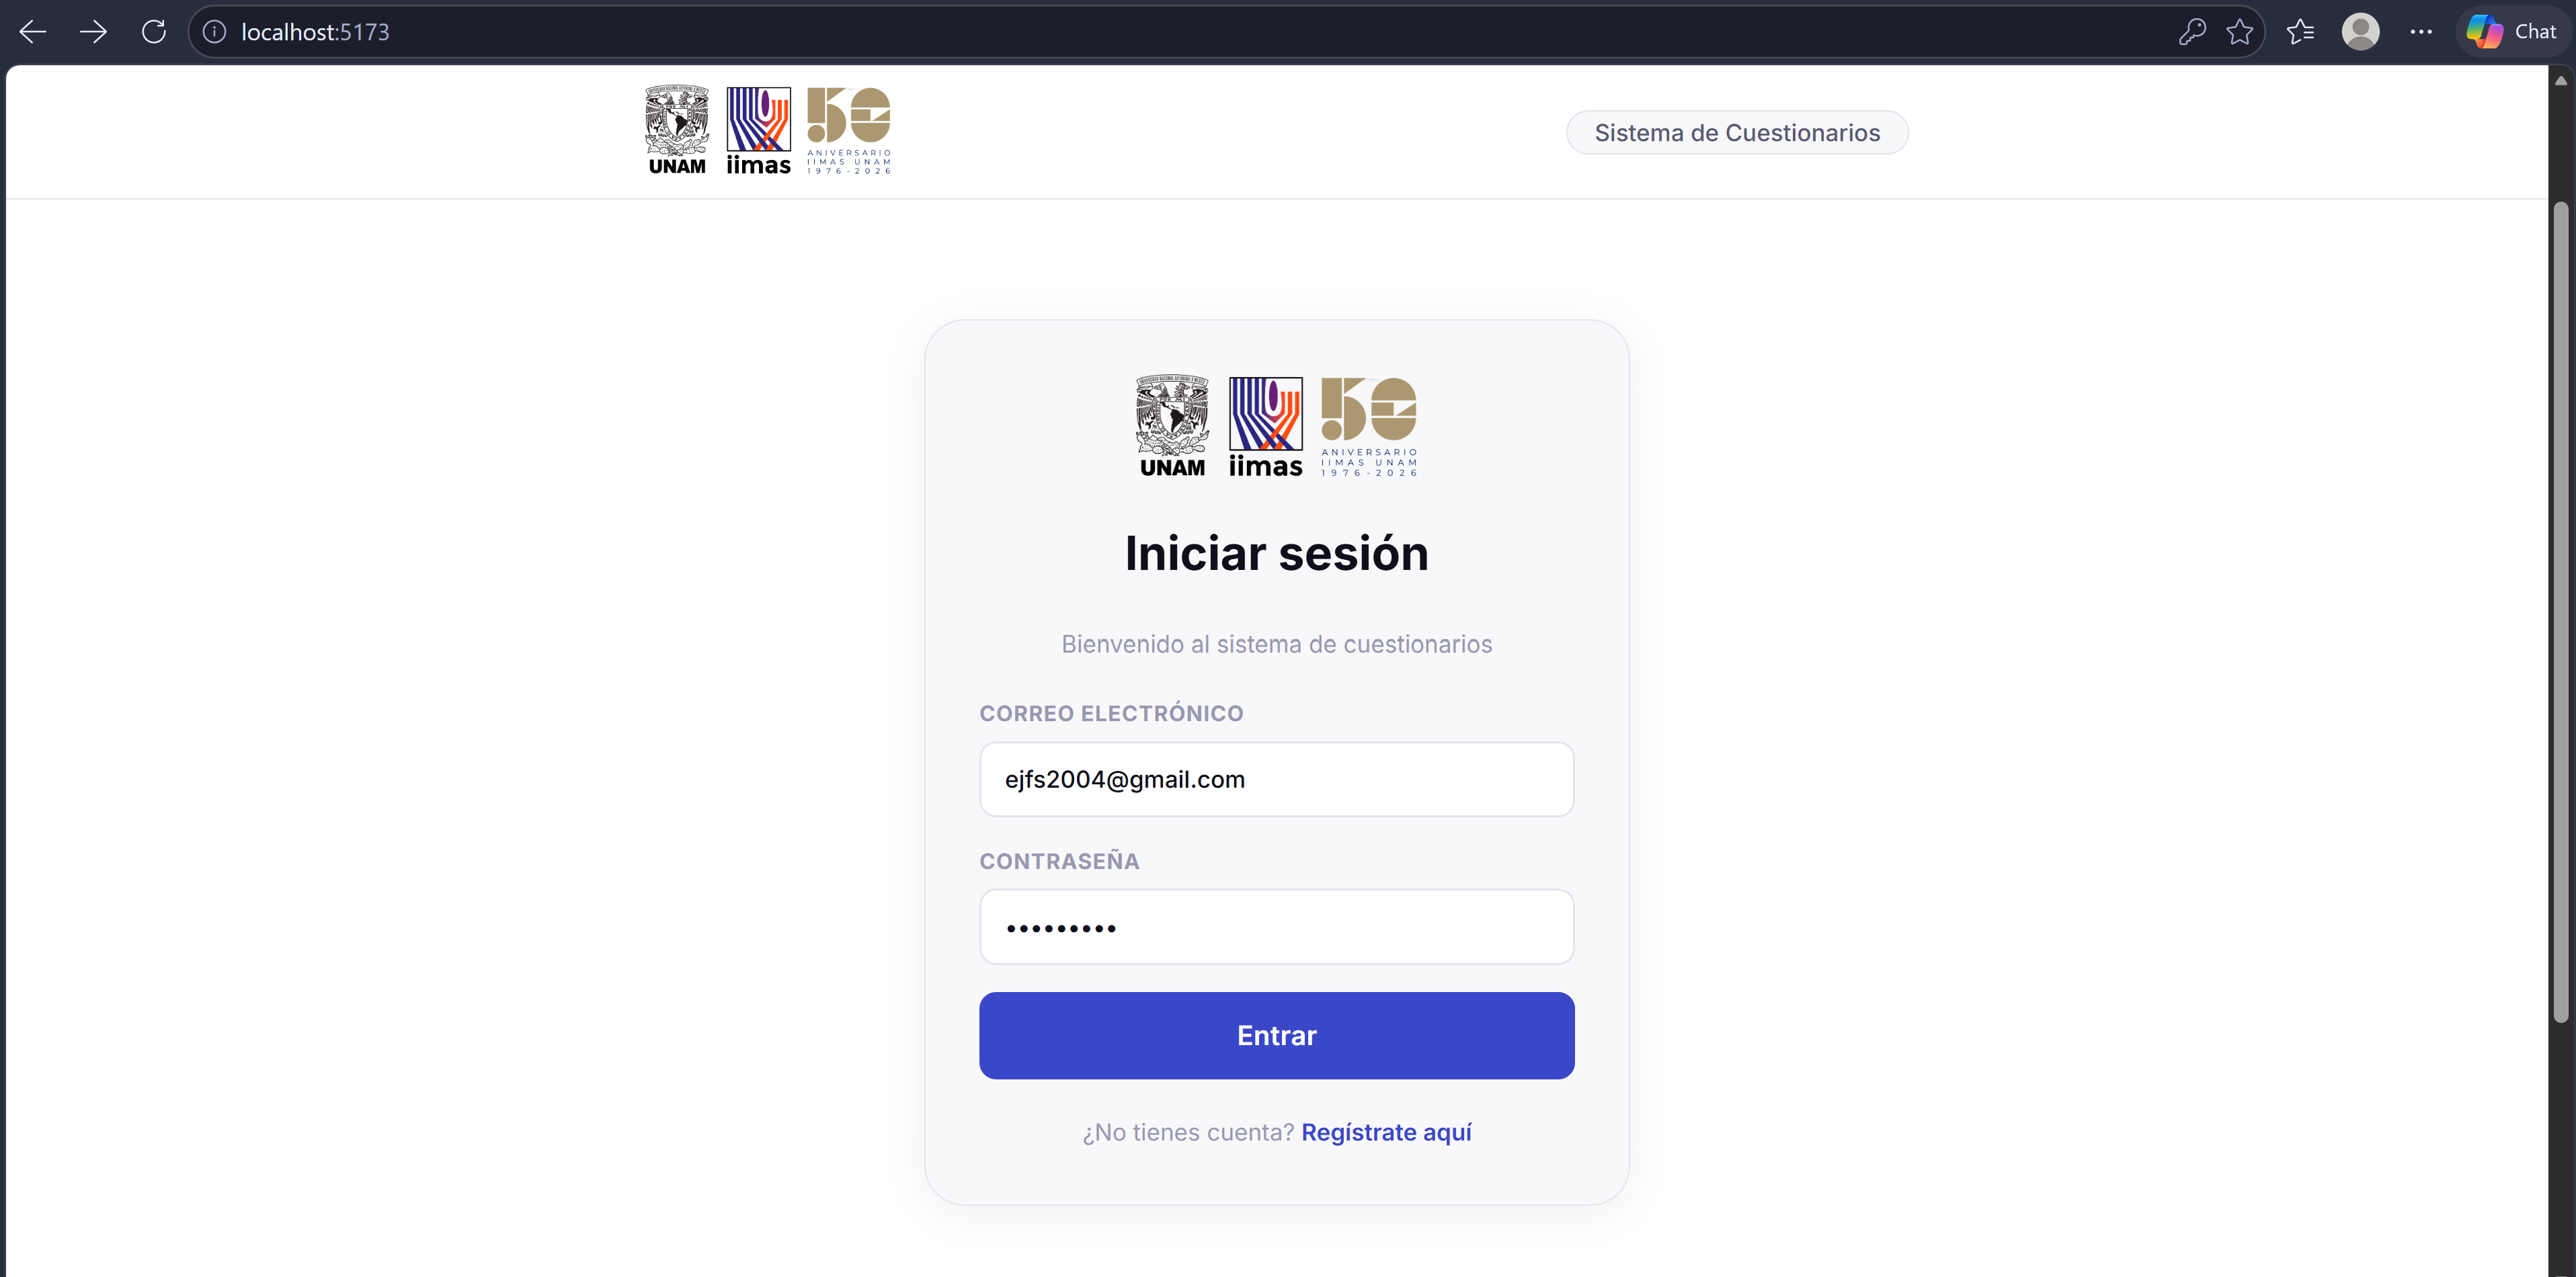
\includegraphics[width=0.75\textwidth]{cap_login.png}
  \caption{Pantalla de inicio de sesión. El usuario ingresa correo y contraseña.}
\end{figure}

Al ingresar a \url{http://localhost:5173} se presenta la pantalla de login. El usuario introduce su correo electrónico y contraseña. Si no tiene cuenta, puede hacer clic en el enlace \textit{Crear cuenta}.

\subsection{Registro de usuario}

\begin{figure}[H]
  \centering
  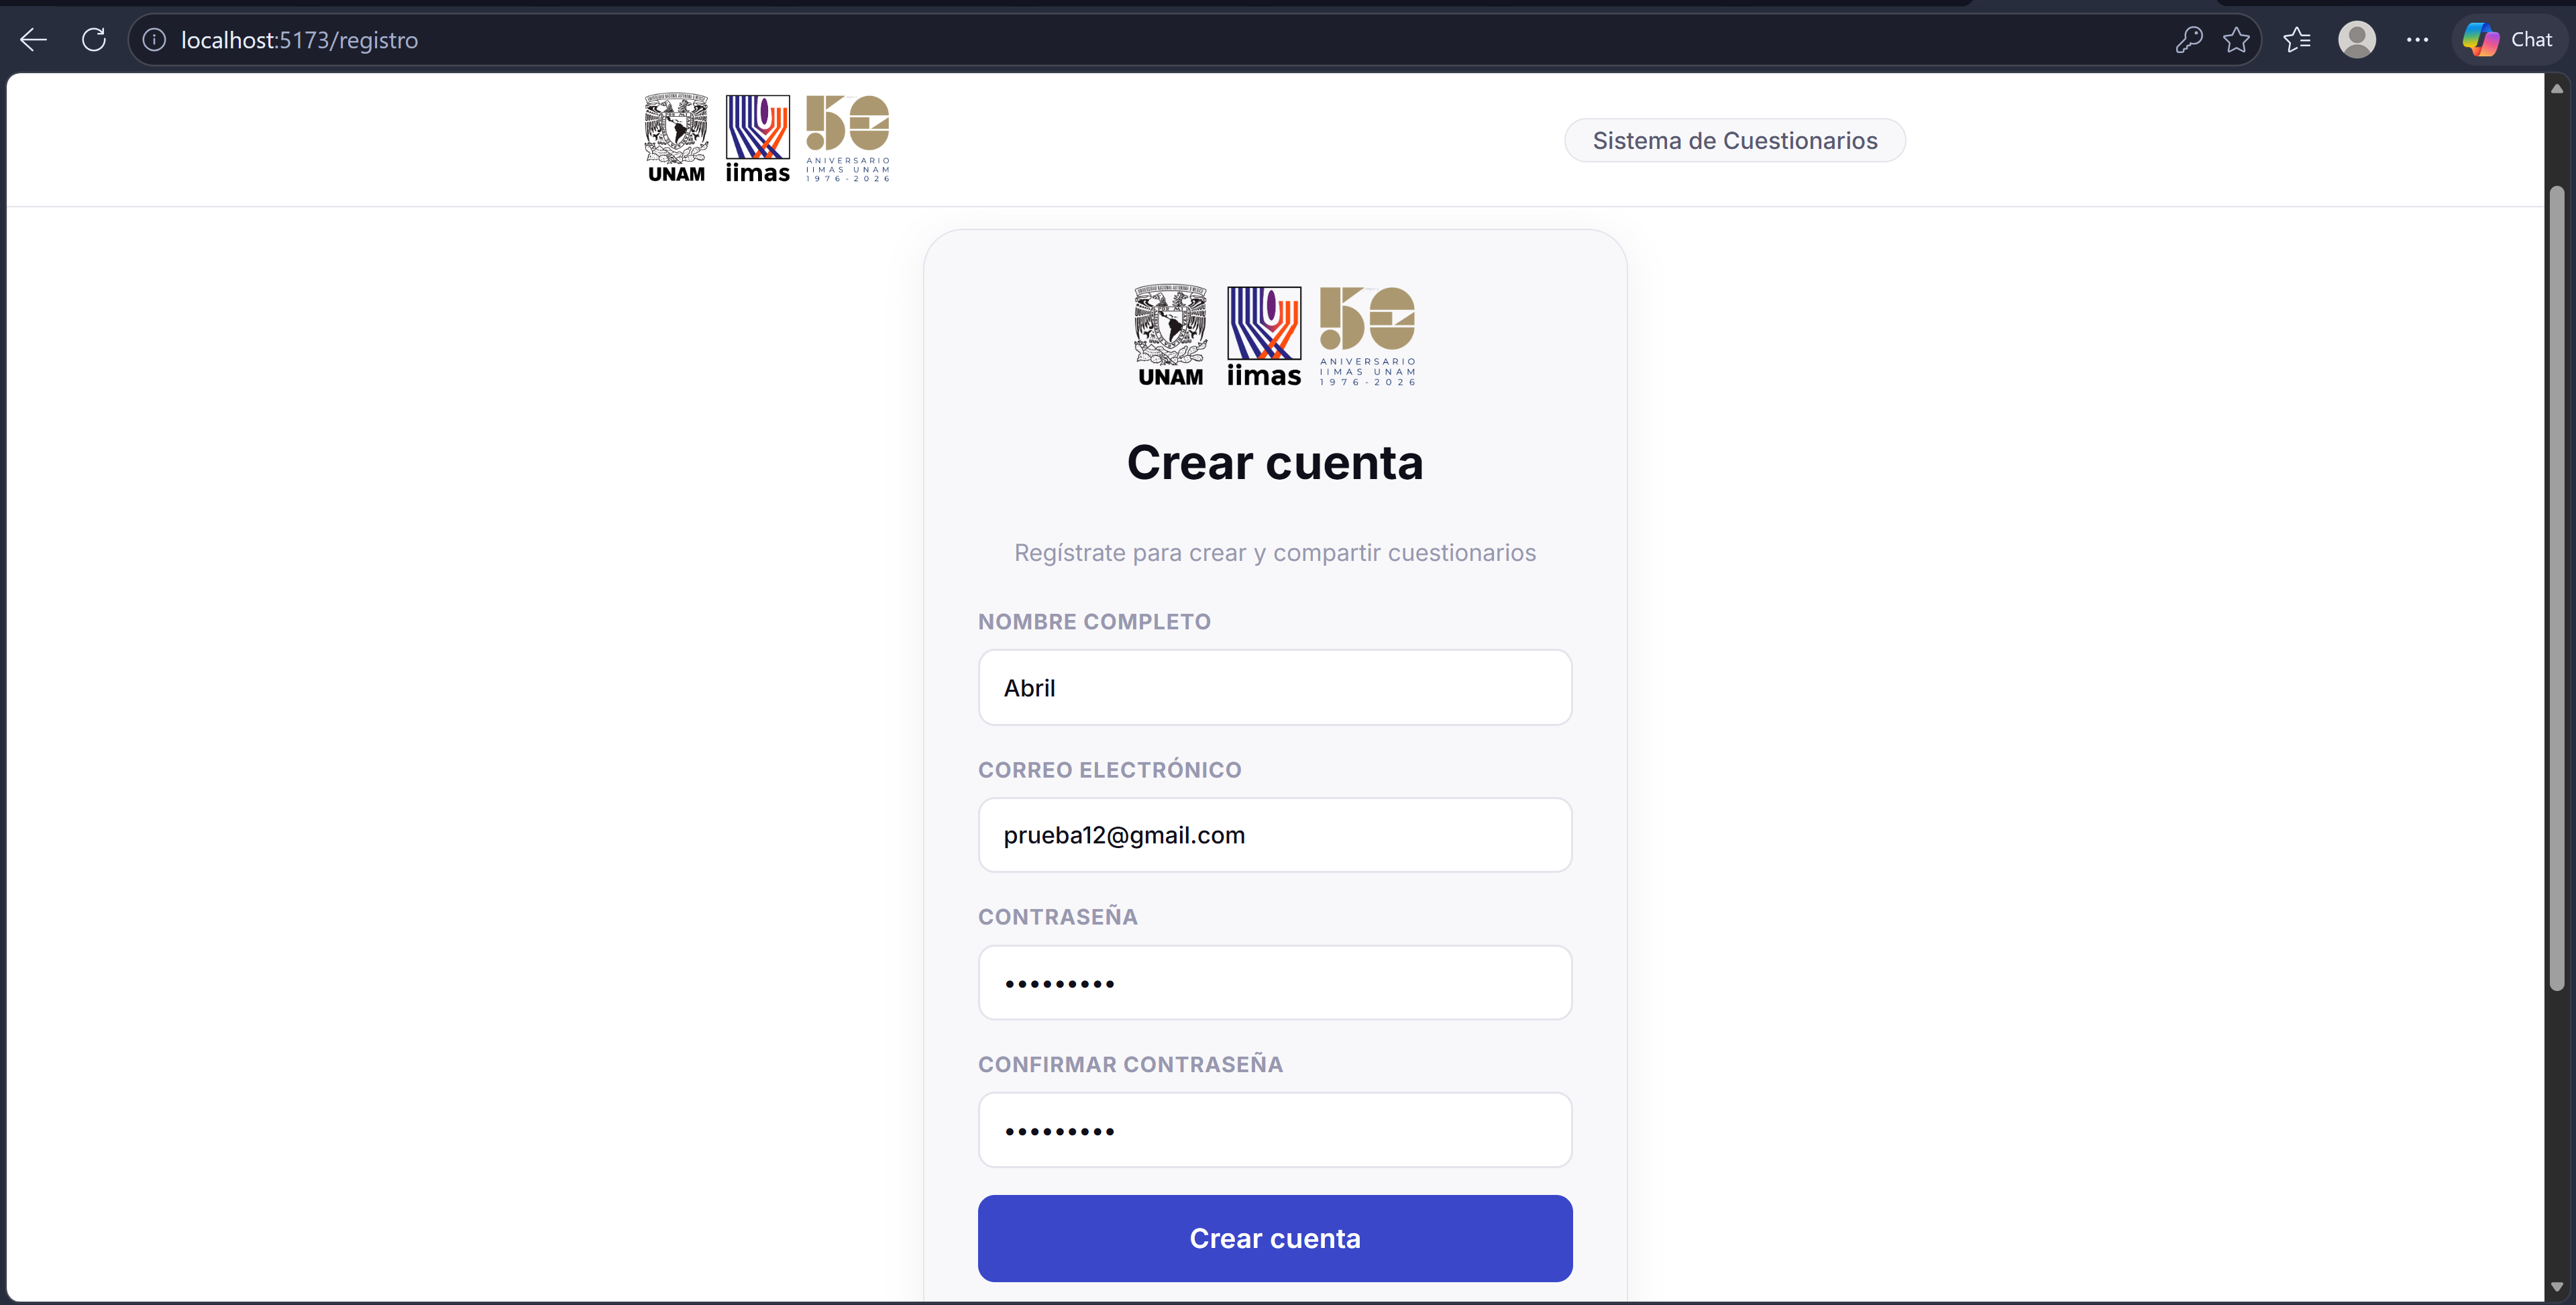
\includegraphics[width=0.75\textwidth]{cap_registro.png}
  \caption{Pantalla de registro de nuevo usuario.}
\end{figure}

El formulario de registro solicita nombre completo, correo electrónico y contraseña (mínimo 6 caracteres). Al registrarse correctamente, el sistema inicia sesión automáticamente y redirige al dashboard.

\subsection{Panel principal (Dashboard)}

\begin{figure}[H]
  \centering
  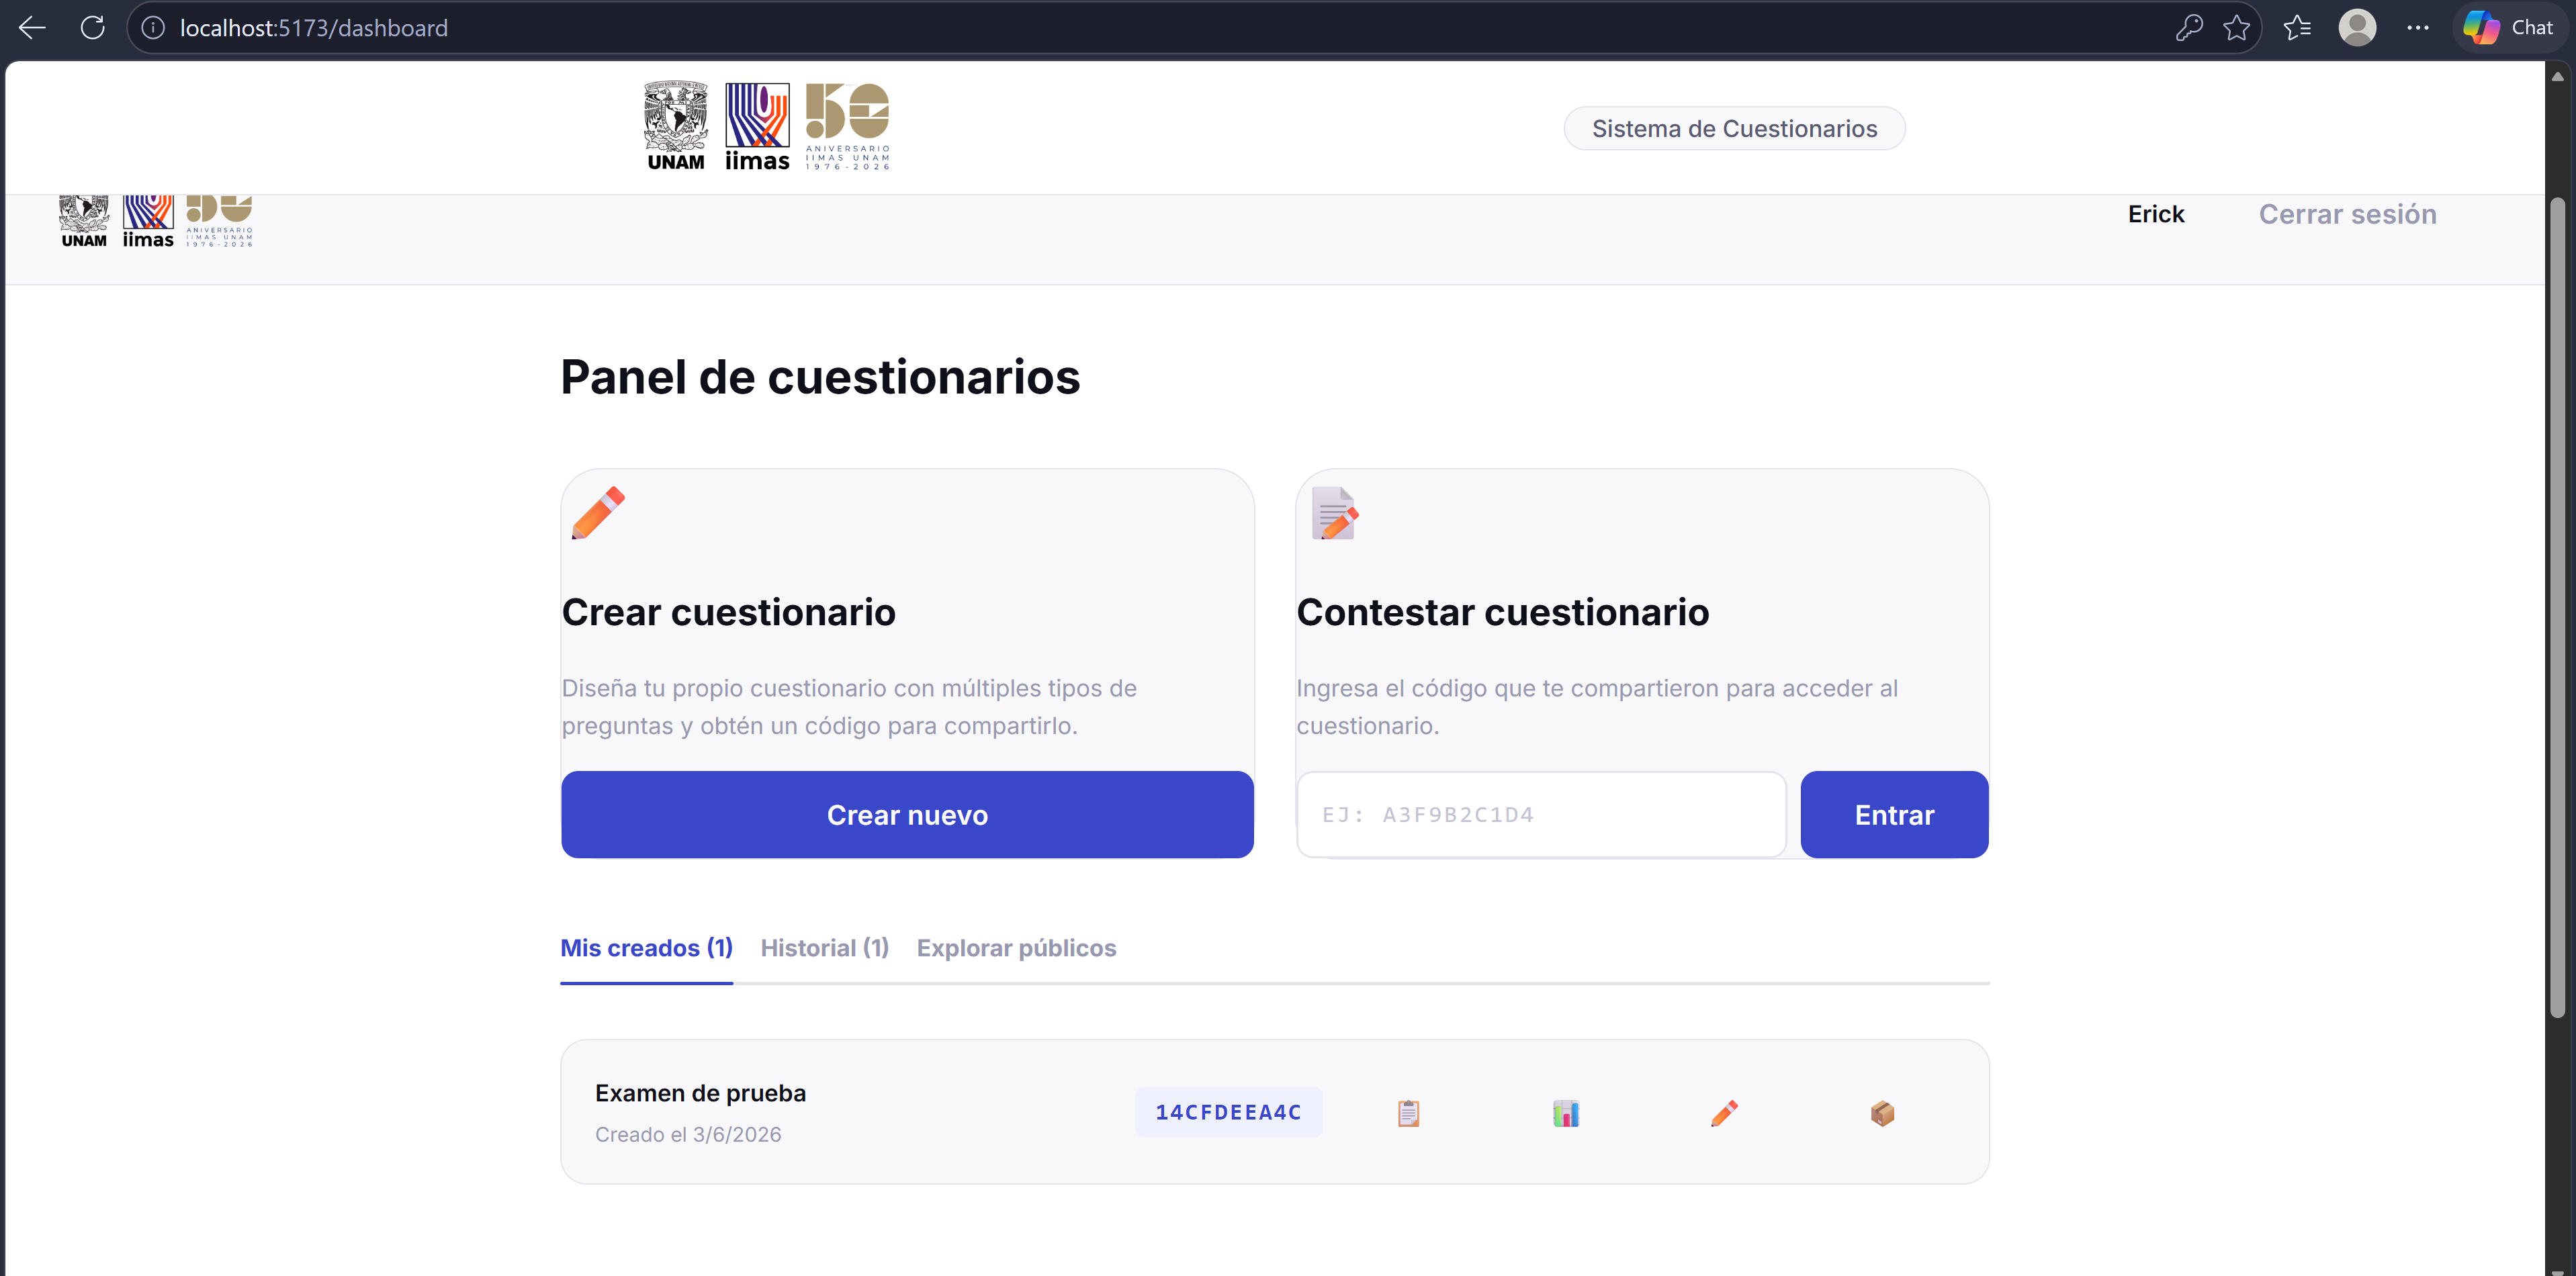
\includegraphics[width=0.9\textwidth]{cap_dashboard.png}
  \caption{Panel principal con las opciones de crear cuestionario, contestar por código y las pestañas de listas.}
\end{figure}

El dashboard muestra:
\begin{itemize}
  \item \textbf{Crear cuestionario:} botón para ir al formulario de creación.
  \item \textbf{Contestar cuestionario:} campo para ingresar el código de 10 caracteres.
  \item \textbf{Mis creados:} lista de cuestionarios creados por el usuario con acciones de resultados~(��), editar~(✏️) y archivar/publicar~(��/��).
  \item \textbf{Historial:} cuestionarios que el usuario ya respondió.
  \item \textbf{Explorar públicos:} todos los cuestionarios públicos disponibles.
\end{itemize}

\subsection{Crear cuestionario}

\begin{figure}[H]
  \centering
  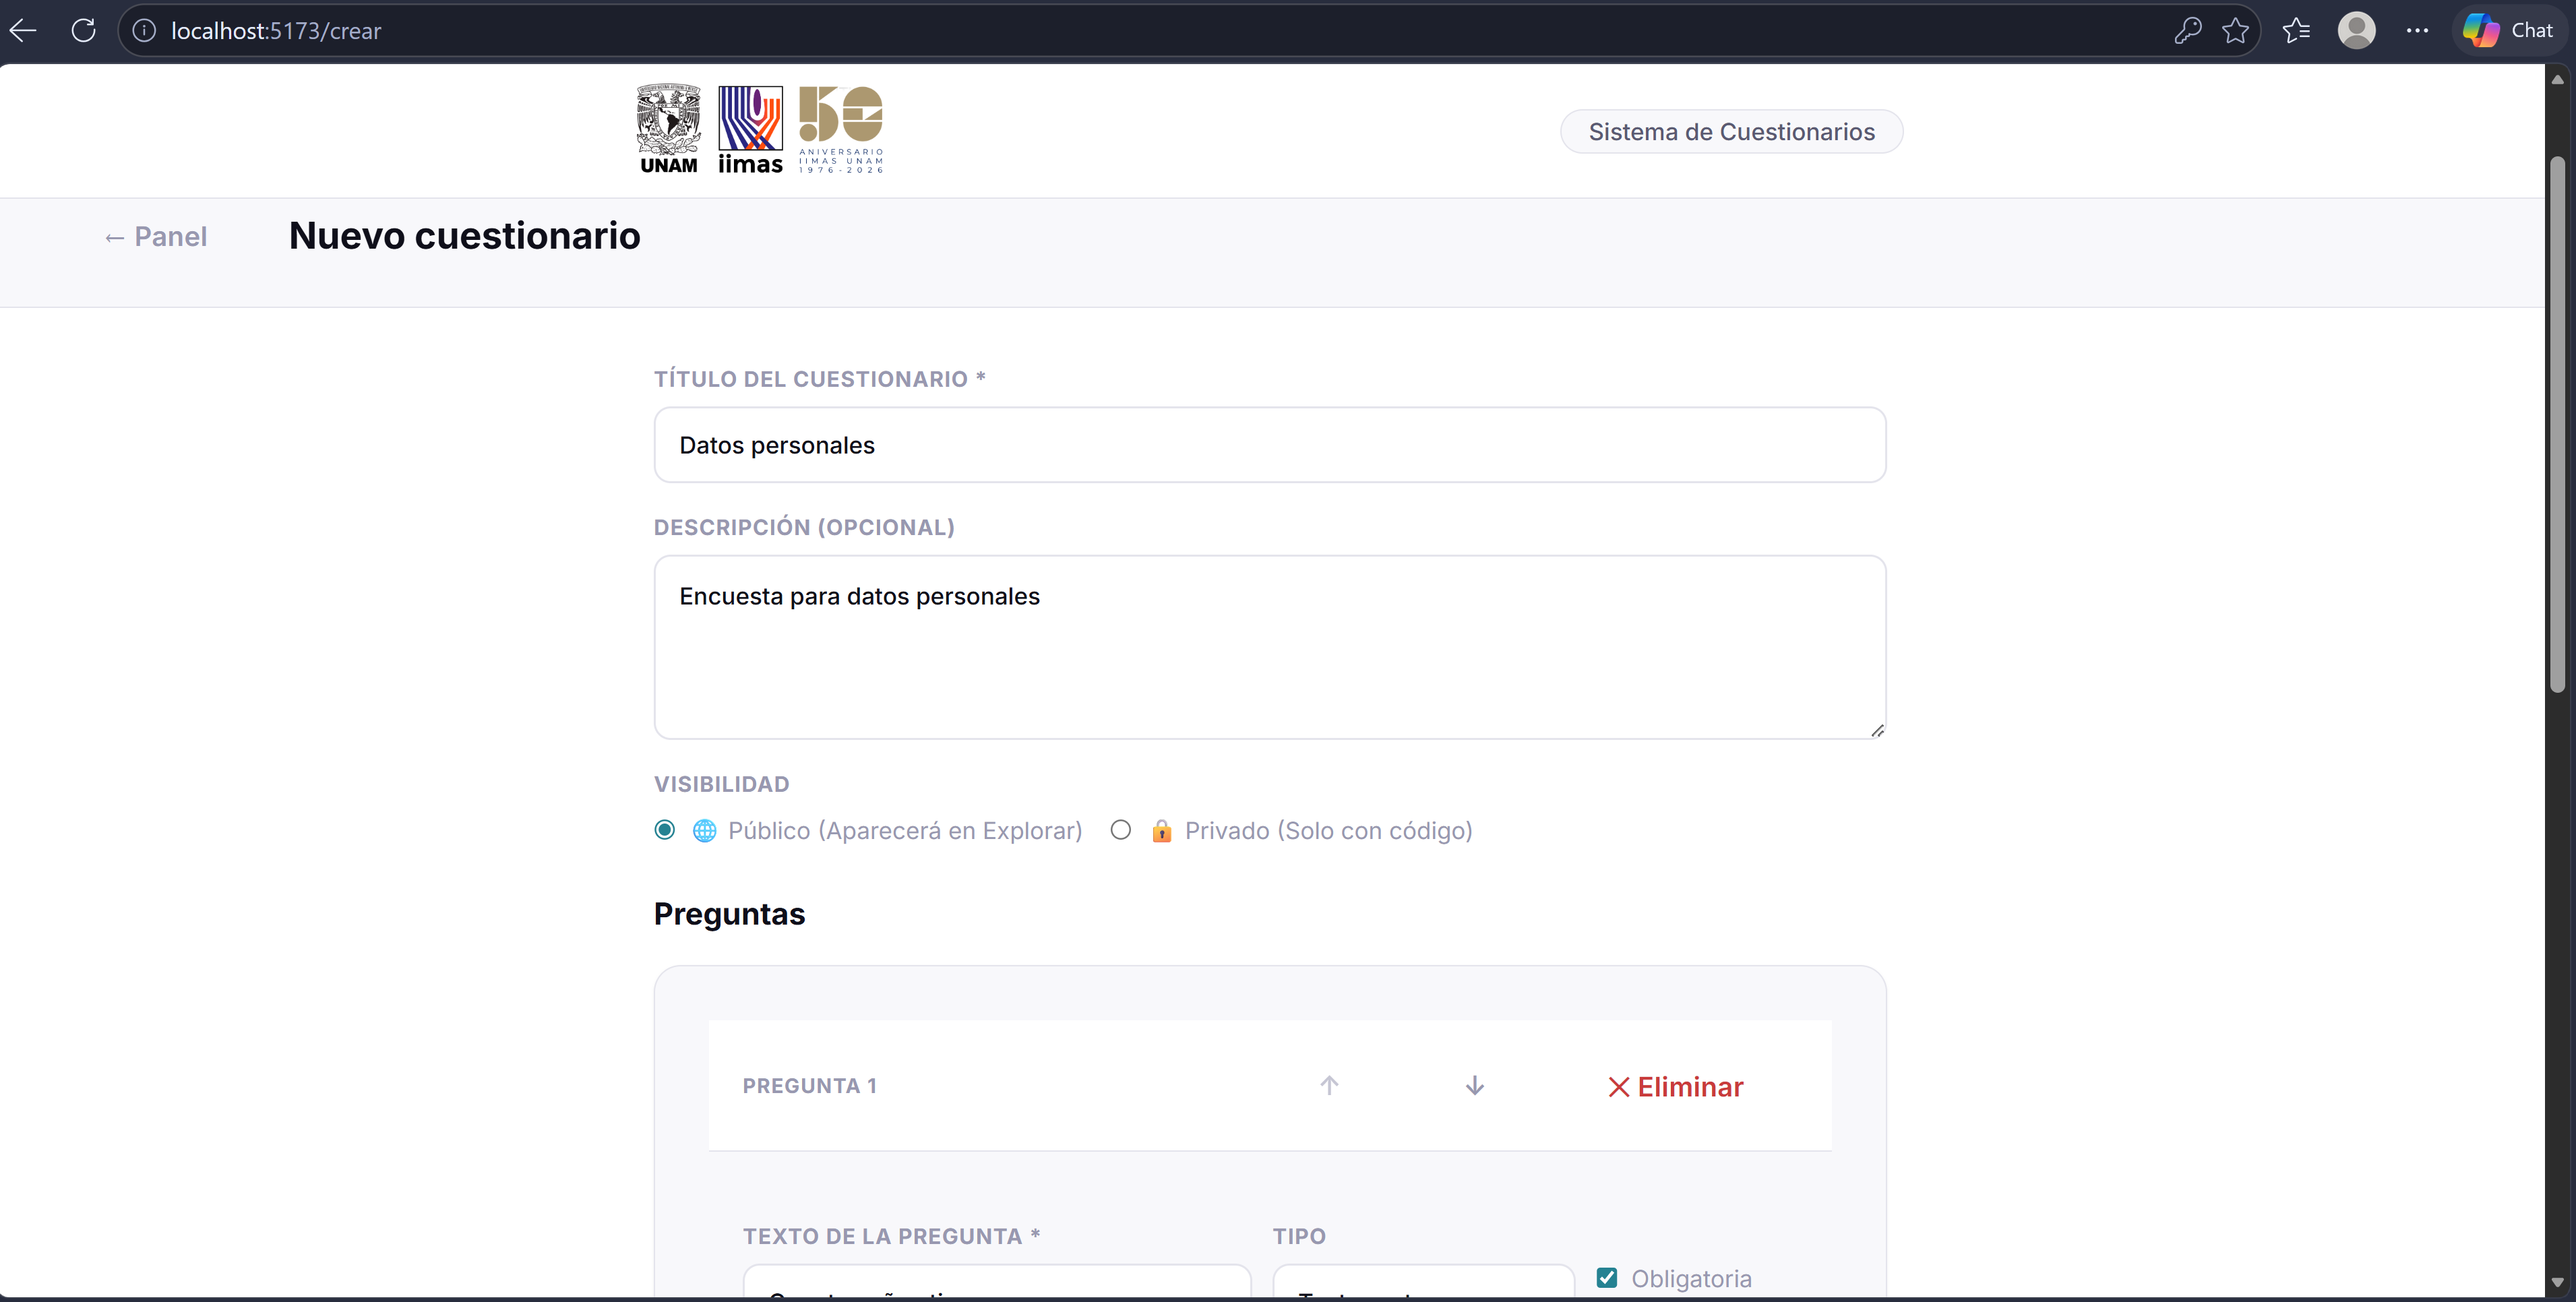
\includegraphics[width=0.9\textwidth]{cap_crear.png}
  \caption{Vista de creación de cuestionario con tipos de pregunta, botones de reordenar y previsualización.}
\end{figure}

El creador puede:
\begin{itemize}
  \item Escribir título, descripción y seleccionar visibilidad (público / privado).
  \item Agregar preguntas de 7 tipos: texto corto, texto largo, opción única, opción múltiple, escala 1--5, Sí/No y fecha.
  \item Reordenar preguntas con los botones \textbf{↑} y \textbf{↓}.
  \item Para los tipos Sí/No, escala y fecha se muestra una previsualización; para opción única/múltiple se agregan las opciones manualmente.
\end{itemize}

\subsection{Contestar cuestionario — Identificación}

\begin{figure}[H]
  \centering
  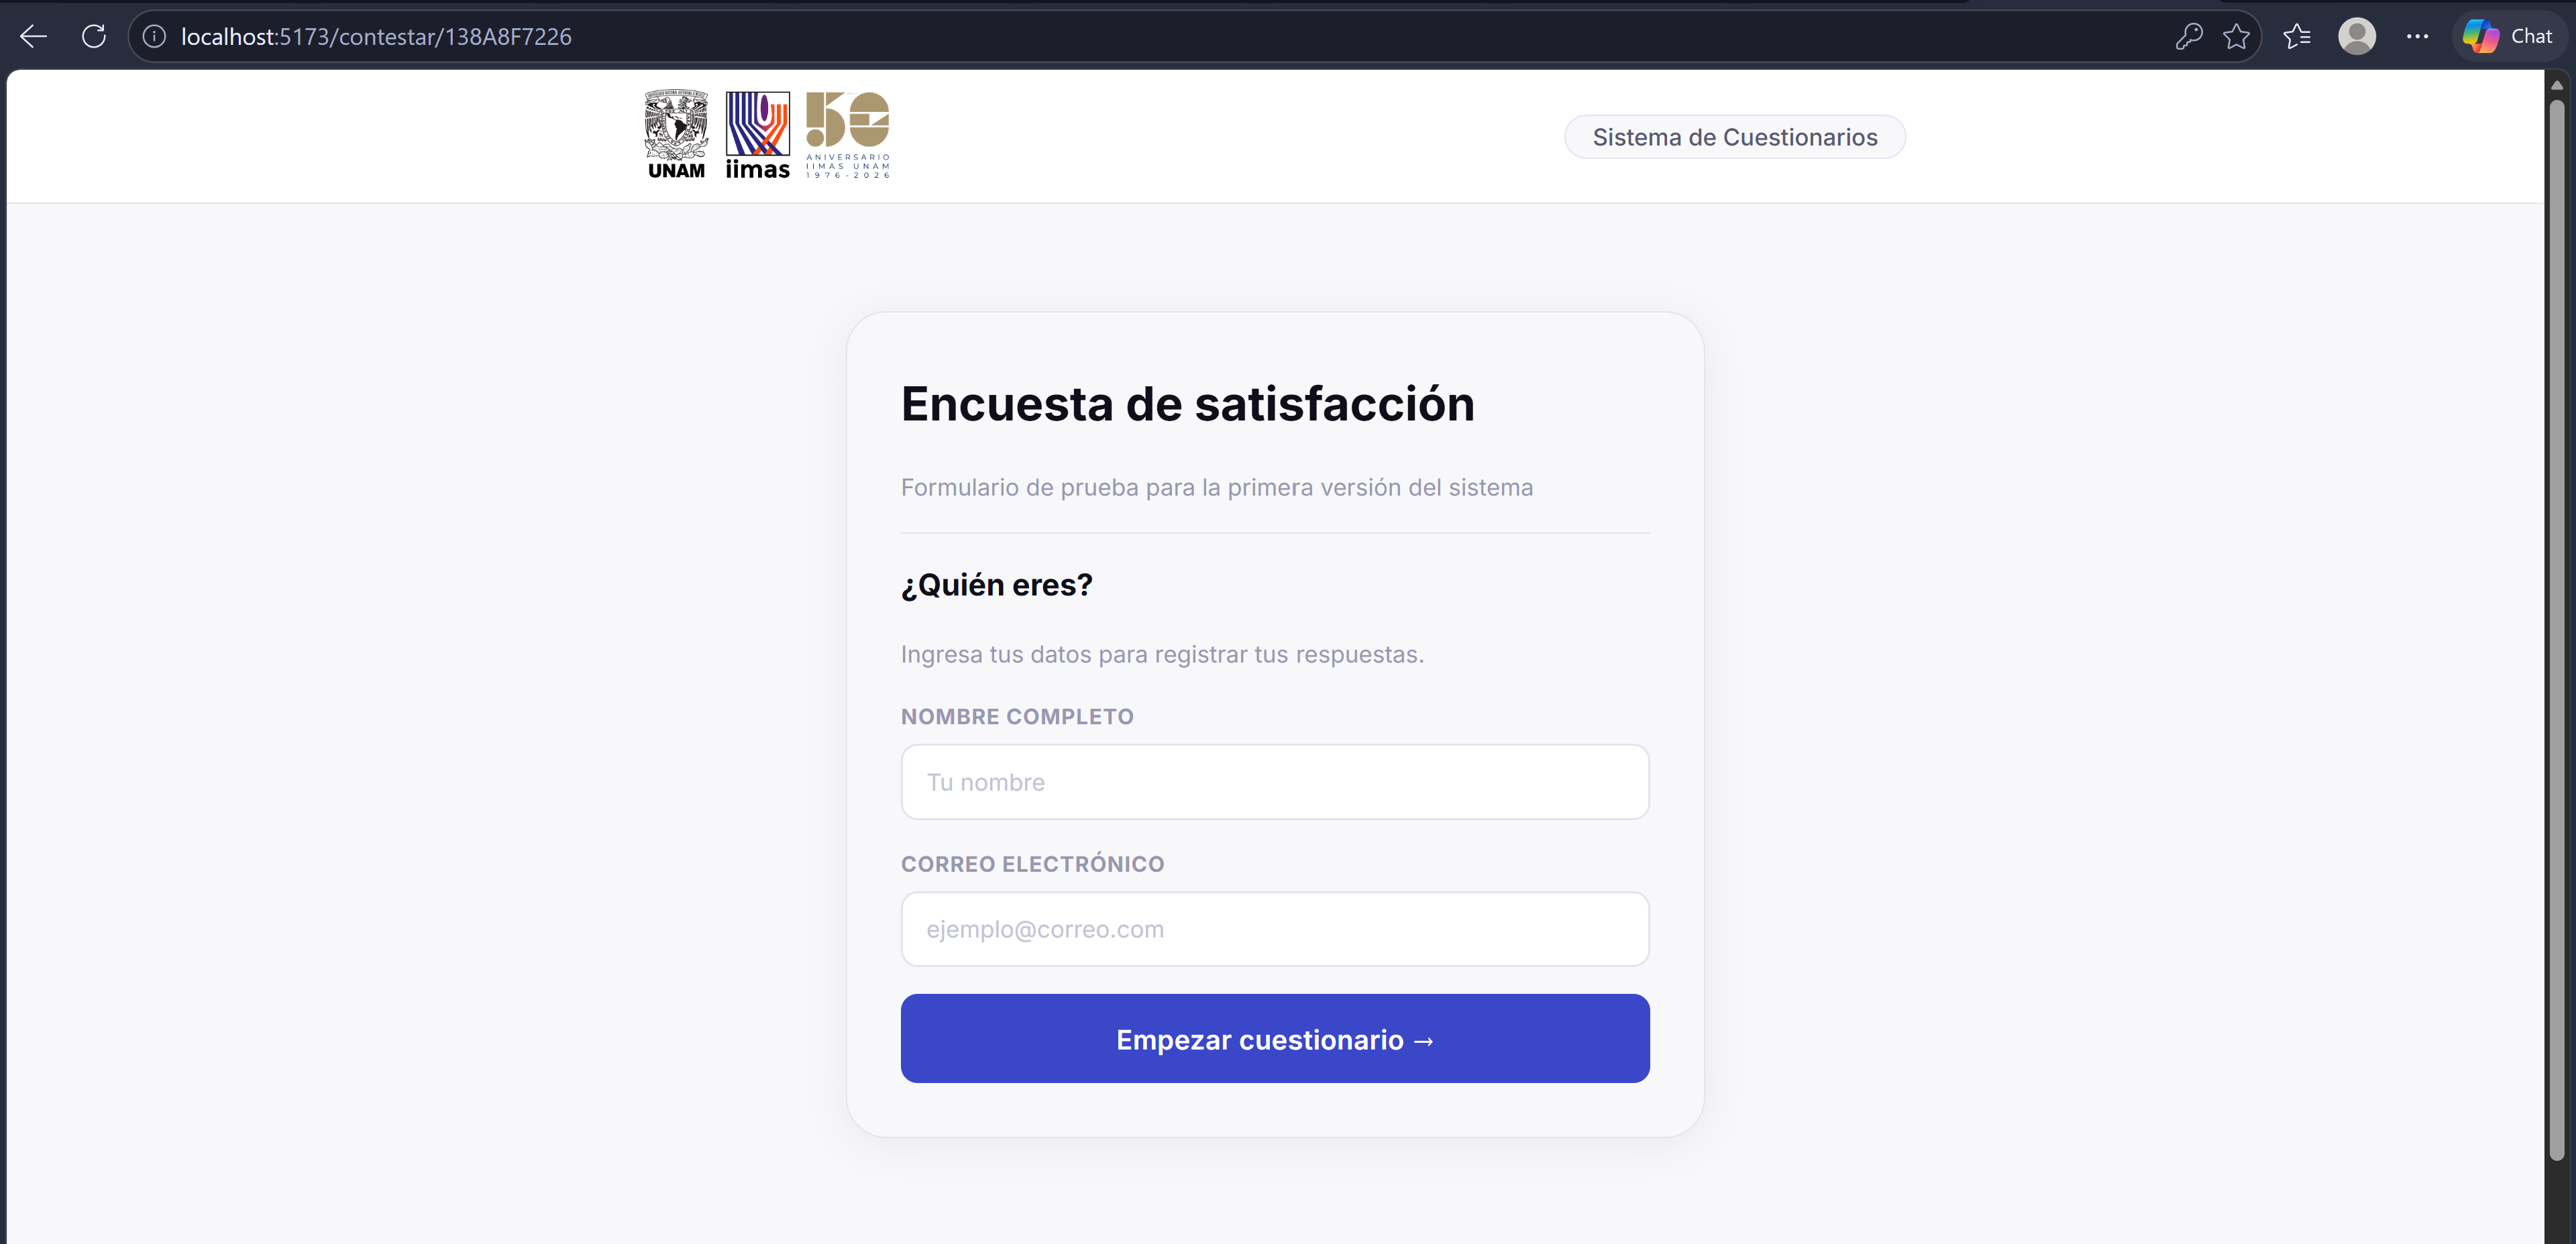
\includegraphics[width=0.75\textwidth]{cap_contestar_id.png}
  \caption{Pantalla de identificación del respondente antes de iniciar el cuestionario.}
\end{figure}

El respondente ingresa el código compartido y luego se identifica con su nombre y correo. El sistema verifica si ya contestó anteriormente y recupera el avance parcial si existe.

\subsection{Contestar cuestionario — Preguntas}

\begin{figure}[H]
  \centering
  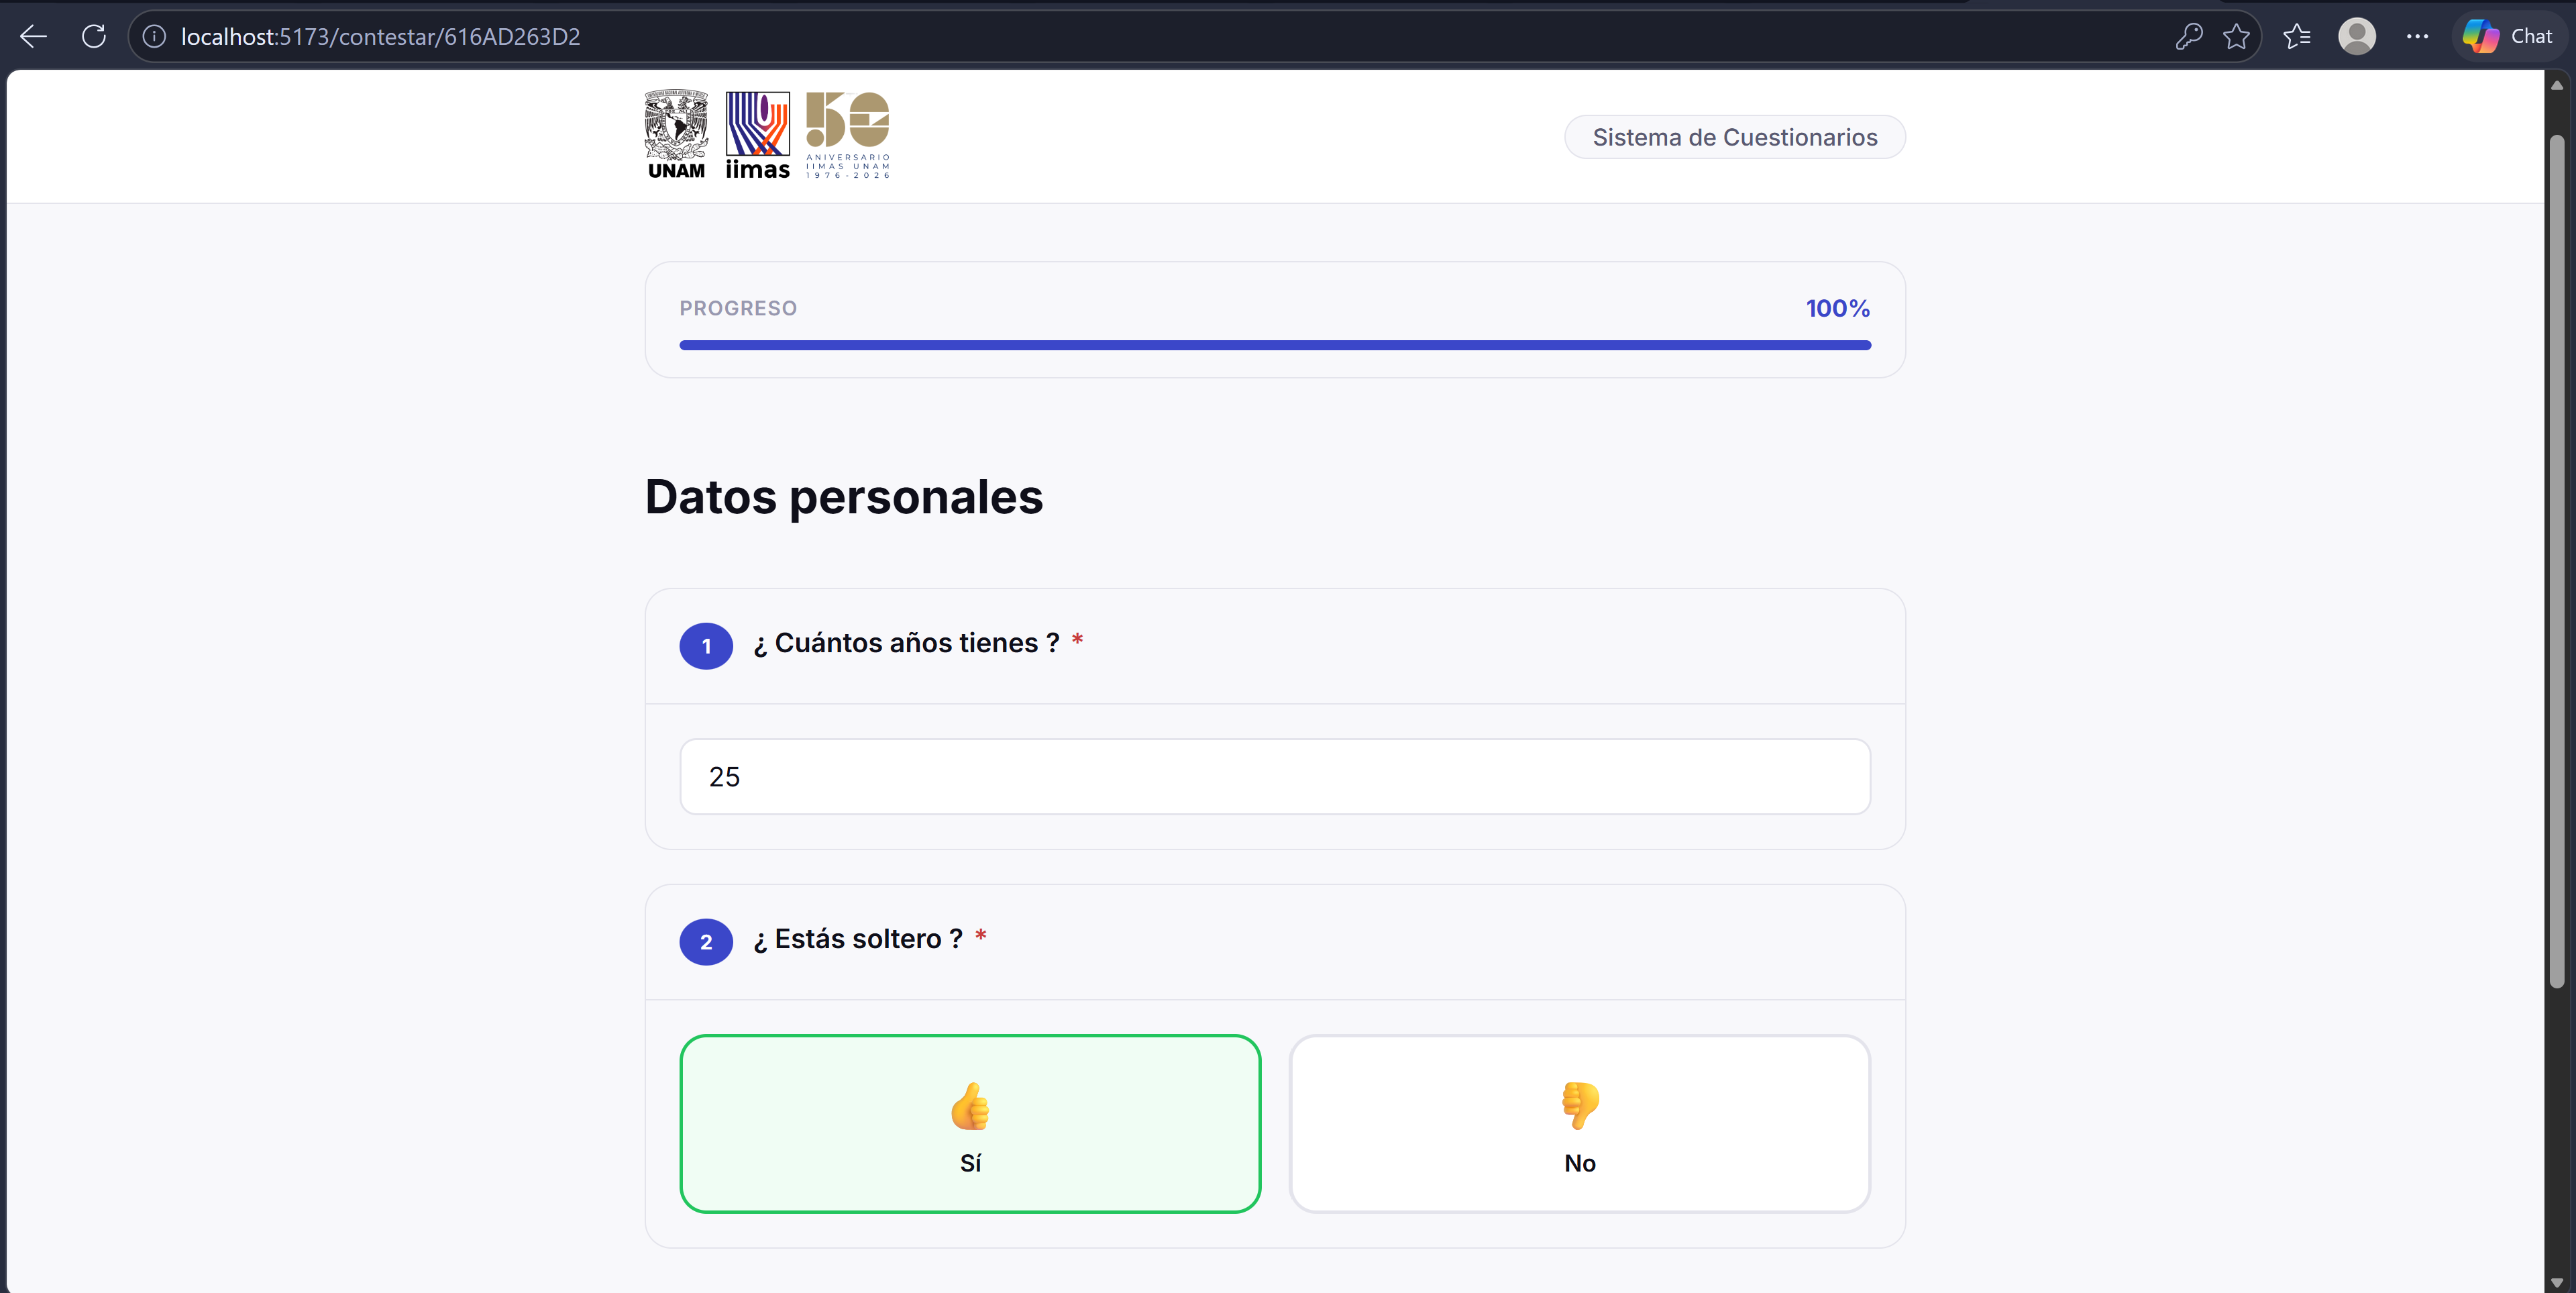
\includegraphics[width=0.9\textwidth]{cap_contestar_preguntas.png}
  \caption{Vista de respuesta con barra de progreso y distintos tipos de pregunta.}
\end{figure}

La vista de respuesta incluye:
\begin{itemize}
  \item Barra de progreso que indica el porcentaje de preguntas respondidas.
  \item Guardado automático al cambiar de pregunta (y al cerrar la pestaña).
  \item Los botones ��/�� para preguntas Sí/No.
  \item Selector de fecha nativo del navegador para preguntas de tipo fecha.
  \item Botón \textit{Enviar respuestas} que valida las preguntas obligatorias antes de guardar.
\end{itemize}

\subsection{Editar cuestionario}

\begin{figure}[H]
  \centering
  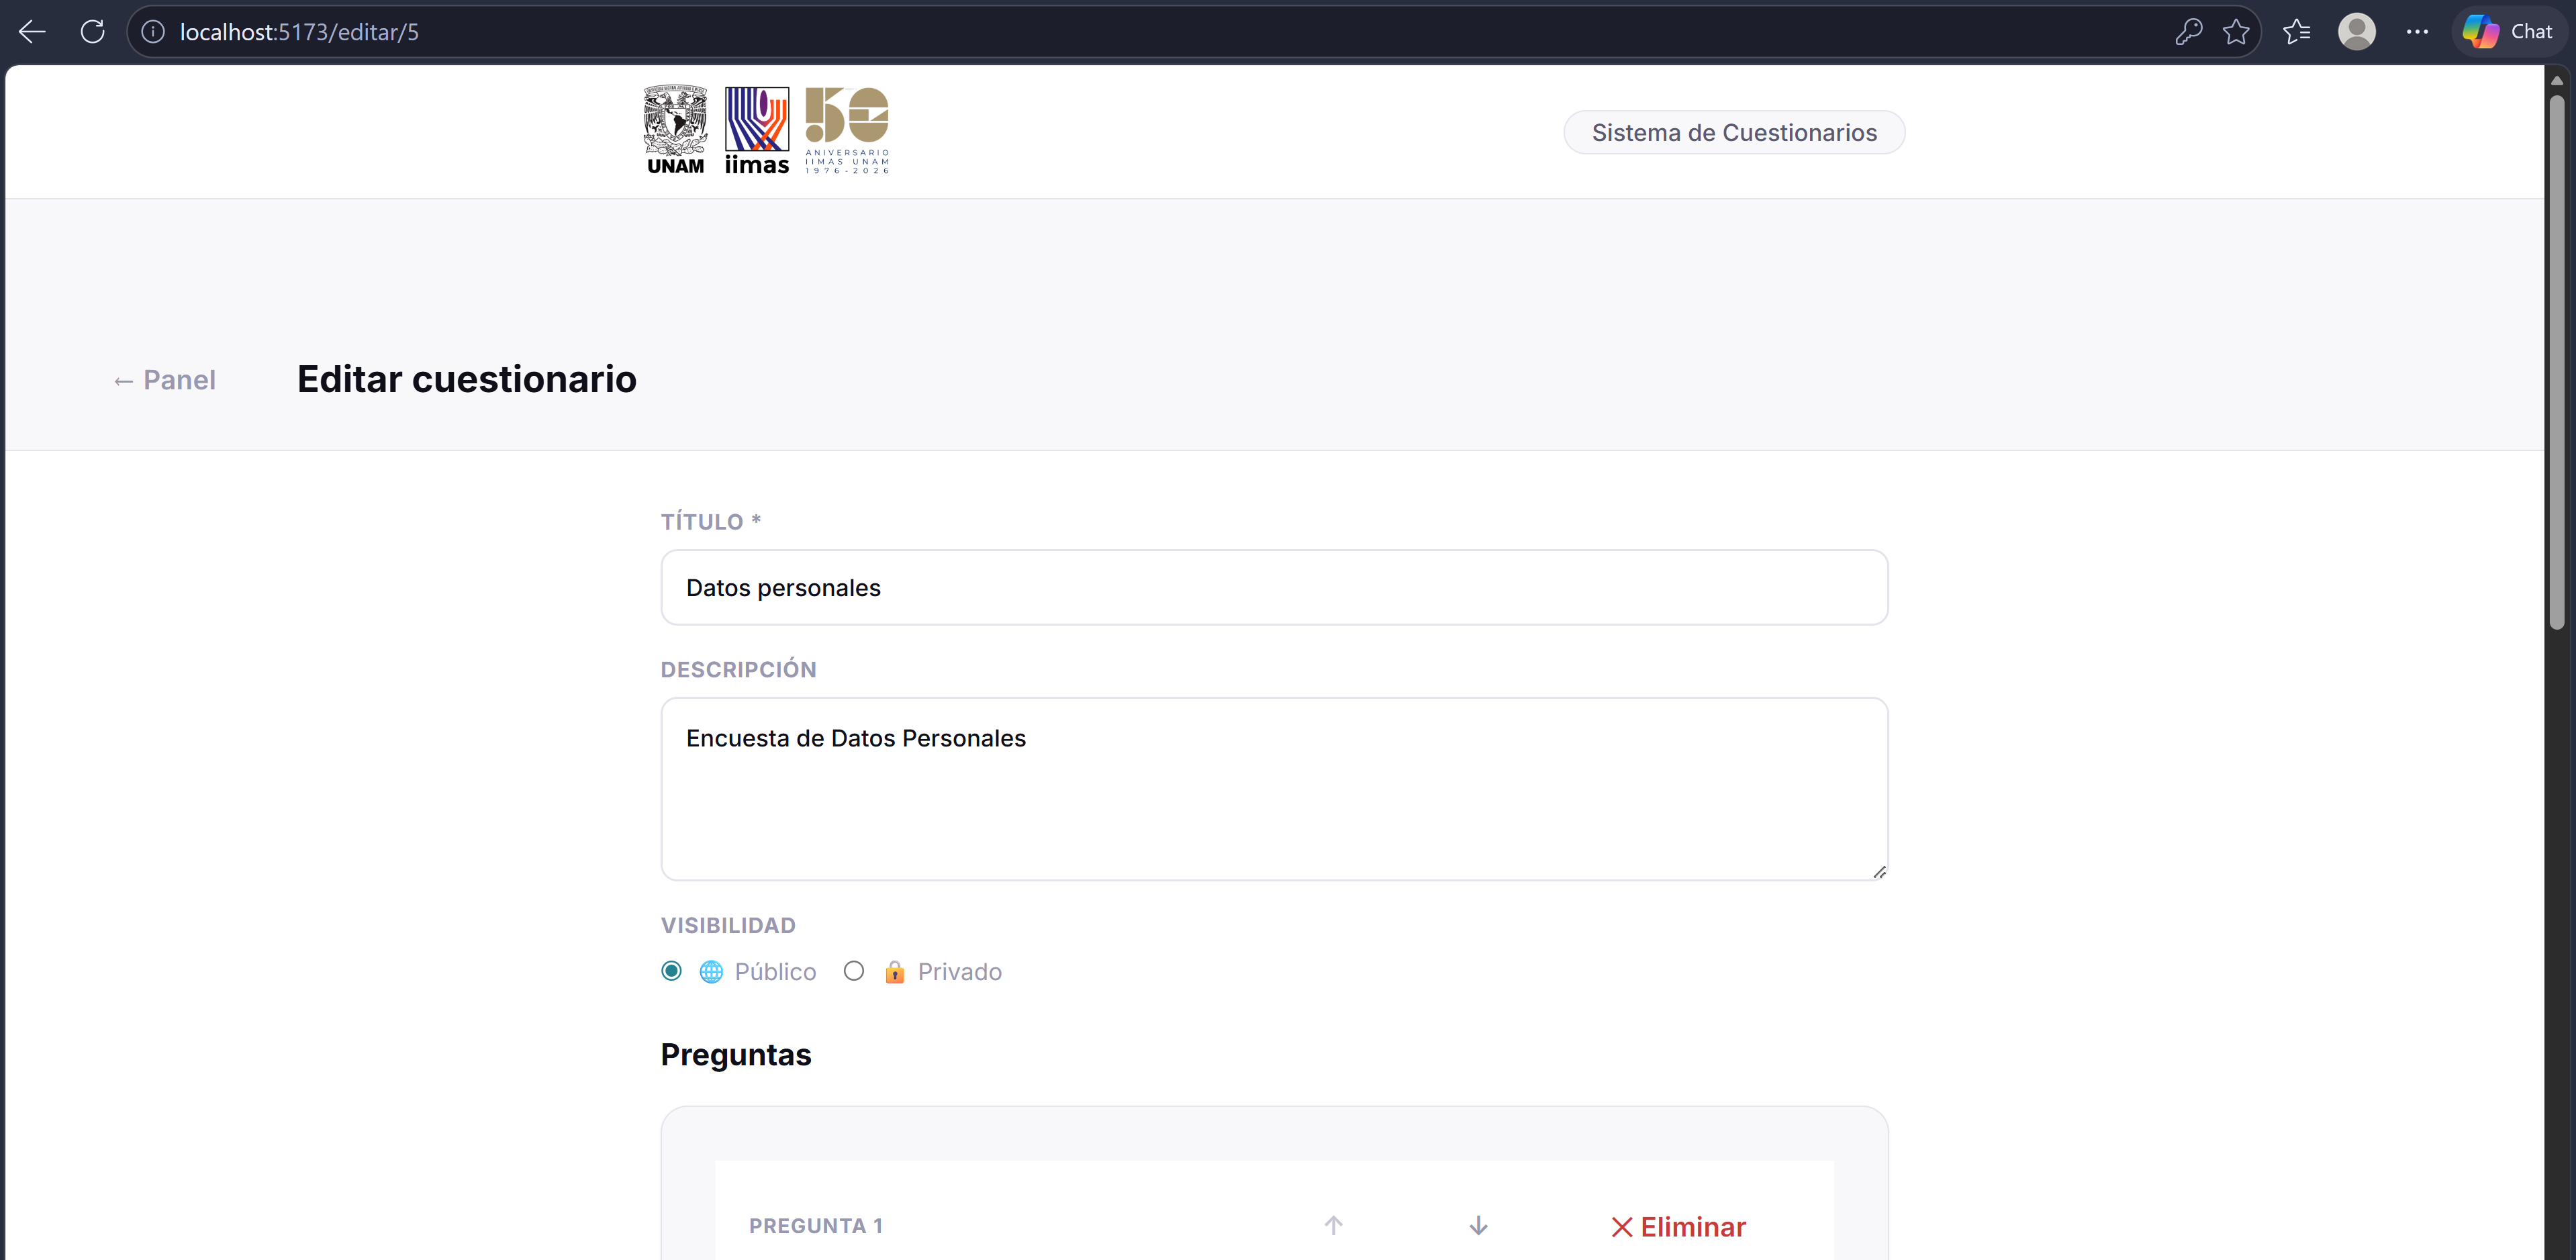
\includegraphics[width=0.9\textwidth]{cap_editar.png}
  \caption{Vista de edición. Si ya existen respuestas, solo se pueden editar los metadatos.}
\end{figure}

Accesible desde el botón ✏️ del dashboard. Permite modificar título, descripción y visibilidad en cualquier momento. La edición de preguntas solo está disponible si el cuestionario no tiene respuestas todavía (el sistema muestra un aviso en caso contrario).

\subsection{Ver resultados}

\begin{figure}[H]
  \centering
  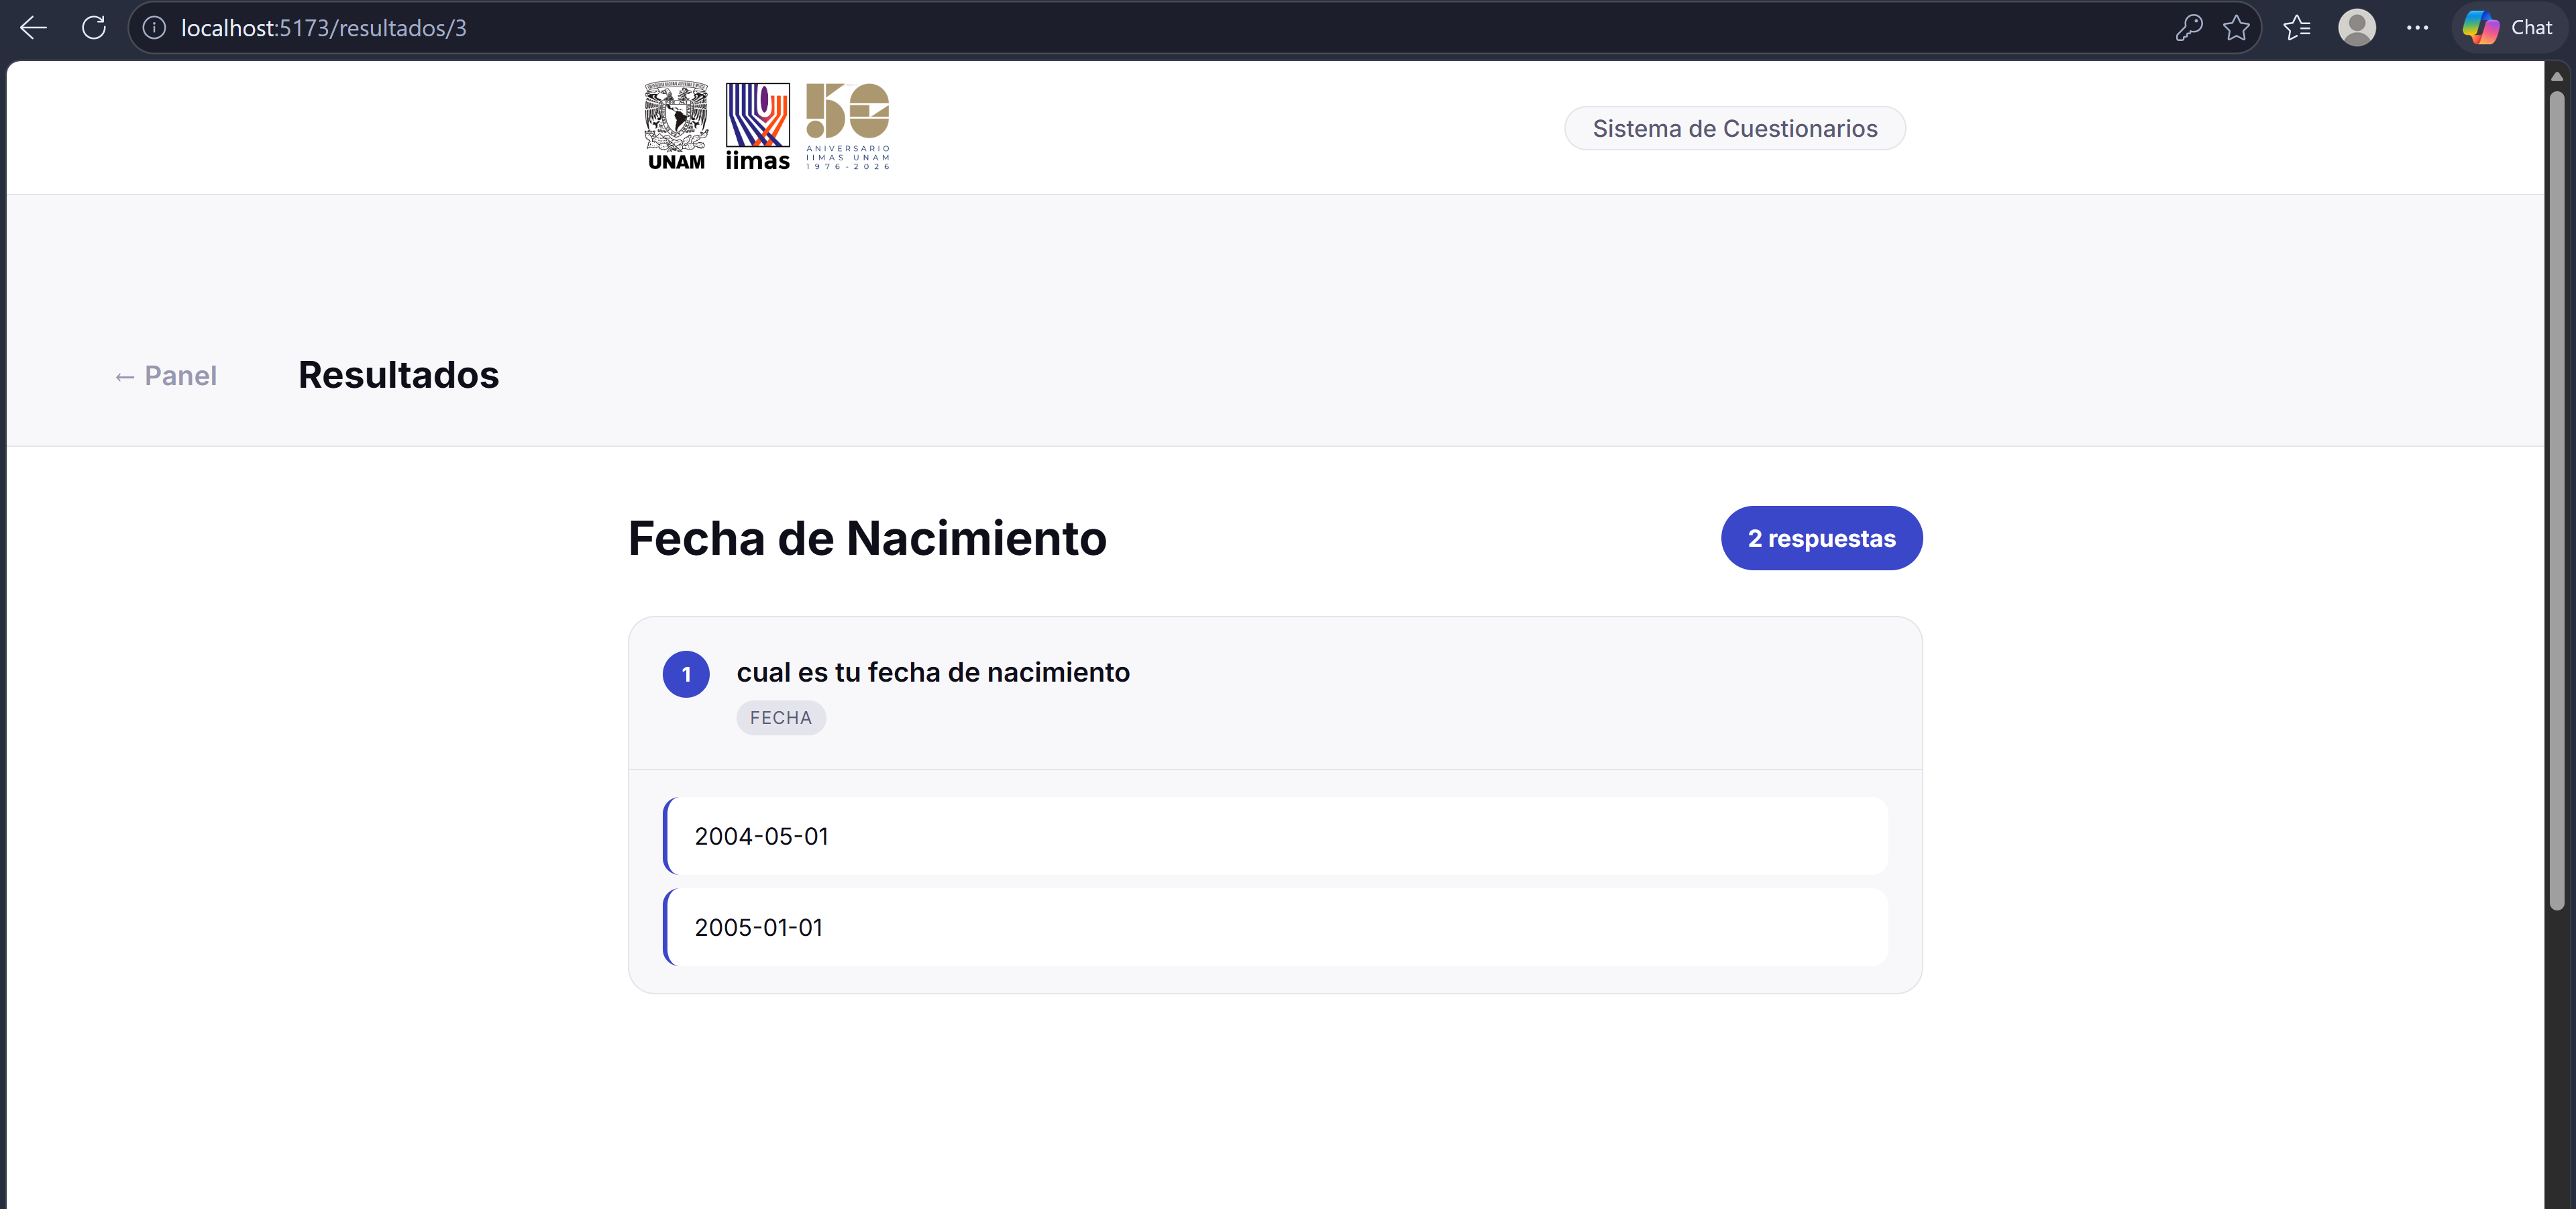
\includegraphics[width=0.9\textwidth]{cap_resultados.png}
  \caption{Vista de resultados con estadísticas por pregunta: barras CSS, promedio de escala y listado de respuestas textuales.}
\end{figure}

Accesible desde el botón �� del dashboard (solo para el creador). Muestra:
\begin{itemize}
  \item Total de respuestas recibidas.
  \item \textbf{Preguntas de texto/fecha:} listado de las respuestas enviadas.
  \item \textbf{Escala:} promedio numérico y distribución por valor (1--5) con barras CSS.
  \item \textbf{Opción única/múltiple/Sí-No:} conteo y porcentaje por opción con barras de progreso (verde para Sí, rojo para No).
\end{itemize}

\subsection{Confirmación de envío}

\begin{figure}[H]
  \centering
  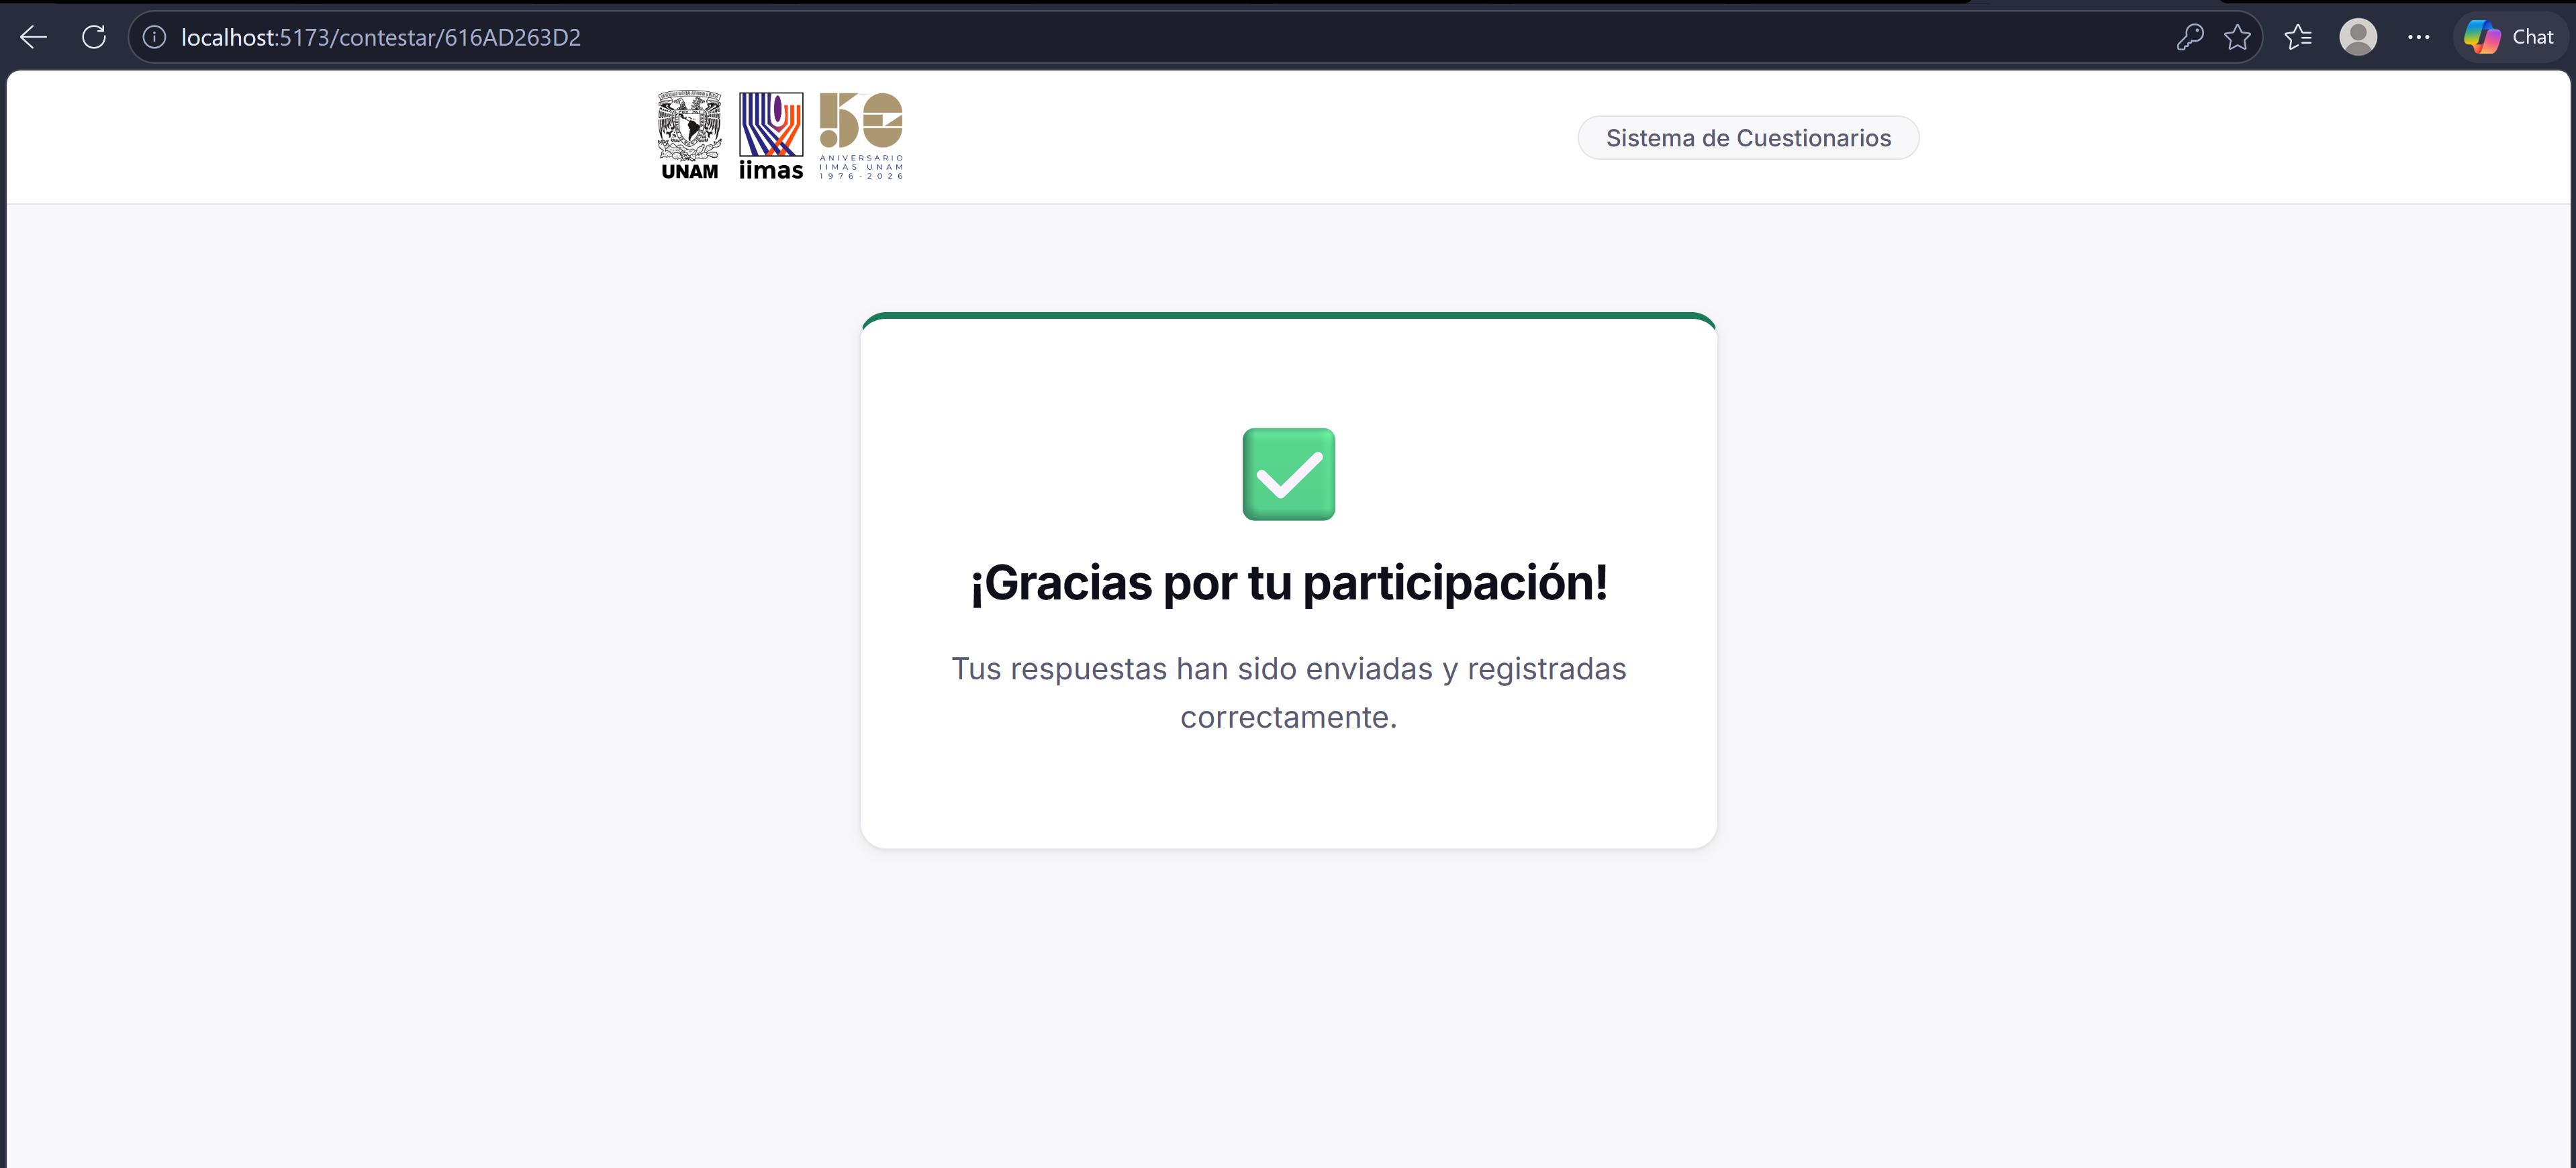
\includegraphics[width=0.65\textwidth]{cap_gracias.png}
  \caption{Pantalla de agradecimiento tras enviar correctamente las respuestas.}
\end{figure}

Tras enviar el cuestionario, el sistema muestra una pantalla de confirmación. El intento queda registrado y el sistema impide que el mismo usuario responda de nuevo.

% =============================================================
\section{Conclusión}
% =============================================================

El proyecto implementa una aplicación web desacoplada completa para la creación y gestión de cuestionarios en línea. El backend Flask expone una API RESTful con autenticación por token, y el frontend Vue 3 consume dicha API de forma independiente.

Las funcionalidades implementadas en esta versión final incluyen: registro e inicio de sesión con contraseña hasheada, creación de cuestionarios con 7 tipos de pregunta, reordenamiento de preguntas, edición de cuestionarios, archivado/publicación, vista de resultados con estadísticas agregadas, guardado automático de avance y diferenciación entre cuestionarios públicos y privados.

El código fuente, historial de cambios y este documento se encuentran disponibles en:

\begin{center}
\url{https://github.com/0ElaLe/AplicacionCuestionarios}
\end{center}

% =============================================================
%  LISTA DE IMÁGENES NECESARIAS PARA OVERLEAF
% =============================================================
% Subir a Overleaf con exactamente estos nombres:
%
%   logo_iimas.png     — Logo del IIMAS (esquina superior izquierda portada)
%   logo_unam.png      — Escudo de la UNAM (esquina superior derecha portada)
%   cap_login.png      — Captura de la pantalla de inicio de sesión
%   cap_registro.png   — Captura de la pantalla de registro de nuevo usuario
%   cap_dashboard.png  — Captura del panel principal completo (con las 3 pestañas visibles)
%   cap_crear.png      — Captura de la vista de crear cuestionario (con al menos 2 preguntas)
%   cap_contestar_id.png      — Captura de la pantalla de identificación al contestar
%   cap_contestar_preguntas.png — Captura del cuestionario siendo respondido
%   cap_editar.png     — Captura de la vista de editar cuestionario
%   cap_resultados.png — Captura de la vista de resultados con estadísticas
%   cap_gracias.png    — Captura de la pantalla de confirmación de envío
% =============================================================

\end{document}
